%%%% ijcai25.tex

\typeout{IJCAI--25 Instructions for Authors}

% These are the instructions for authors for IJCAI-25.

\documentclass{article}
\pdfpagewidth=8.5in
\pdfpageheight=11in

% The file ijcai25.sty is a copy from ijcai22.sty
% The file ijcai22.sty is NOT the same as previous years'
\usepackage{ijcai25}

% Use the postscript times font!
\usepackage{times}
\usepackage{soul}
\usepackage{url}
\usepackage[hidelinks]{hyperref}
\usepackage[utf8]{inputenc}
\usepackage[small]{caption}
\usepackage{graphicx}
\usepackage{amsmath}
\usepackage{amsthm}
\usepackage{booktabs}
\usepackage{algorithm}
%\usepackage{algorithmic}
\usepackage[switch]{lineno}
\usepackage{algpseudocode}

\usepackage{amssymb}
\usepackage{macros}
\usepackage{mathrsfs}
\usepackage{tikz}
\usepackage{bussproofs}
\usetikzlibrary{shapes.misc, fit, decorations.pathreplacing,calligraphy,positioning} %for crossing-out arrows and rectangles around nodes

\usepackage{soul}
\usepackage{todonotes}
\newcommand\rustam[1]{\todo[color=blue!30,size=\small,inline]{Rustam: #1}}
\newcommand\davide[1]{\todo[color=green!30,size=\small,inline]{Davide: #1}}
\newcommand{\rev}[1]{{\color{blue} #1}}
 %\newcommand{\rev}[1]{{#1}}
 \newcommand{\rem}[1]{{\color{red} #1}}

 
\renewcommand{\sl}{\mathfrak{sl}}
 \algtext*{EndIf}
\algtext*{EndFor}

\algnewcommand\algorithmiccase{\textbf{case}}
\algdef{SE}[CASE]{Case}{EndCase}[1]{\algorithmiccase\ #1}{\algorithmicend\ \algorithmiccase}%
\algtext*{EndCase}



% Comment out this line in the camera-ready submission
%\linenumbers

\urlstyle{same}

% the following package is optional:
%\usepackage{latexsym}

% See https://www.overleaf.com/learn/latex/theorems_and_proofs
% for a nice explanation of how to define new theorems, but keep
% in mind that the amsthm package is already included in this
% template and that you must *not* alter the styling.
\newtheorem{example}{Example}
\newtheorem{theorem}{Theorem}
\newtheorem{definition}{Definition}
\newtheorem{proposition}{Proposition}
\newtheorem{corollary}{Corollary}
\newtheorem{remark}{Remark}
\newtheorem{lemma}{Lemma}

% Following comment is from ijcai97-submit.tex:
% The preparation of these files was supported by Schlumberger Palo Alto
% Research, AT\&T Bell Laboratories, and Morgan Kaufmann Publishers.
% Shirley Jowell, of Morgan Kaufmann Publishers, and Peter F.
% Patel-Schneider, of AT\&T Bell Laboratories collaborated on their
% preparation.

% These instructions can be modified and used in other conferences as long
% as credit to the authors and supporting agencies is retained, this notice
% is not changed, and further modification or reuse is not restricted.
% Neither Shirley Jowell nor Peter F. Patel-Schneider can be listed as
% contacts for providing assistance without their prior permission.

% To use for other conferences, change references to files and the
% conference appropriate and use other authors, contacts, publishers, and
% organizations.
% Also change the deadline and address for returning papers and the length and
% page charge instructions.
% Put where the files are available in the appropriate places.


% PDF Info Is REQUIRED.

% Please leave this \pdfinfo block untouched both for the submission and
% Camera Ready Copy. Do not include Title and Author information in the pdfinfo section
\pdfinfo{
/TemplateVersion (IJCAI.2025.0)
}

\title{First-Order Coalition Logic%\thanks{This is an extended version of the paper with the same title that appears in the proceedings of IJCAI
%2025. This version contains a technical appendix with proof details that, for space reasons, do not appear in the IJCAI 2025 version.}
}

%\thanks{This is an extended version of the paper with the same title that appears in the proceedings of IJCAI
%2025. This version contains a technical appendix with proof details that, for space reasons, do not appear in the IJCAI 2025 version.}
% Single author syntax
%\author{
 %   Author Name
  %  \affiliations
   % Affiliation
    %\emails
    %email@example.com
%}

% Multiple author syntax (remove the single-author syntax above and the \iffalse ... \fi here)
%\iffalse
\author{
Davide Catta$^1$
\and
Rustam Galimullin$^2$\And
Aniello Murano$^{3}$\\
\affiliations
$^1$LIPN, CNRS UMR 7030, Université Sorbonne Paris Nord,
  Villetaneuse, France\\
$^2$University of Bergen, Norway\\
$^3$University of Naples Federico II, Italy\\
\emails
catta@lipn.univ-paris13.fr, rustam.galimullin@uib.no, 
aniello.murano@unina.it 
%third@other.example.com,
}
%\fi

\begin{document}

\maketitle

\begin{abstract}
We introduce \textit{First-Order Coalition Logic} ($\CSL$), which combines key intuitions behind Coalition Logic ($\mathsf{CL}$) and Strategy Logic ($\mathsf{SL}$). Specifically, $\CSL$ allows for arbitrary quantification over actions of 
%groups of 
agents.  %The motivation behind $\CSL$ is two-fold. 
$\CSL$ is interesting for several reasons. First, we show that $\CSL$ is strictly more expressive than existing coalition logics. %, and then we study its complexity. 
Second, we provide a sound and complete axiomatisation of $\CSL$, which, to the best of our knowledge, is %represents 
\textit{the first axiomatisation} of any variant of $\mathsf{SL}$ in the literature. %Hence, our work serves as a foundational step towards providing axiomatisations of various strategy logics --- a research question that has been open since the inception of the field.   
Finally, while discussing the satisfiability problem for $\CSL$, we reopen the question of the recursive axiomatisability of $\mathsf{SL}$.
\end{abstract}

\section{Introduction}
\textit{Logics for strategic reasoning} constitute a numerous family of formal tools devised to model, verify, and reason about the abilities and strategies of (groups of) autonomous agents in a competitive environment~\cite{pauly02,alur02,van2005logic,mogavero14,chatterjee2010strategy}. Strategies here are ‘recipes’ telling agents what to do in order to achieve their goals. The competitive environment part arises from the fact that in the presence of several agents trying to achieve their own goals, the actions of one agent may influence the available strategies of another agent. Such logics have been shown to be invaluable for specification and verification within various domains: neuro-symbolic reasoning \cite{akintunde20}, voting protocols \cite{jamroga18}, autonomous submarines \cite{ezekiel11}, manufacturing robots \cite{desilva17}, and so on. 

The prime representatives of logics for strategic reasoning are \textit{coalition logic} ($\mathsf{CL}$) \cite{pauly02}, \textit{alternating-time temporal logic} ($\mathsf{ATL}$), \cite{alur02}, and \textit{strategy logic} ($\mathsf{SL}$) \cite{mogavero10} (and numerous variations thereof). $\mathsf{CL}$ extends the language of propositional logic with constructs $\langle \! \langle C \rangle \! \rangle \varphi$ meaning `coalition $C$ has a joint action such that $\varphi$ holds in the next state (no matter what agents outside of the coalition do at the same time)'. $\mathsf{ATL}$ extends further the abilities of agents to force temporal goals expressed with the help of such modalities as `\textsf{U}ntil' and `\textsf{R}elease'. Finally, $\mathsf{SL}$ allows for a more fine-tuned quantification over agents' abilities: while in both $\mathsf{CL}$ and $\mathsf{ATL}$ we have a fixed quantification prefix $\exists \forall$, in $\mathsf{SL}$ we can have arbitrary quantification prefixes. Thus, in $\mathsf{SL}$ we can reason, for example, about agents sharing their strategies, and such game-theoretic notions like dominant strategies and Nash equilibria.  Hence, $\mathsf{ATL}$ is strictly more expressive than $\mathsf{CL}$, and, in turn, $\mathsf{SL}$ is strictly more expressive than $\mathsf{ATL}$ (and its more general cousin $\mathsf{ATL}^\ast$).

%The incredible expressivity of $\mathsf{SL}$ comes at a price: the complexity of the model checking for $\mathsf{SL}$ is non-elementary, and it remains quite high for different fragments as well \cite{mogavero14}. Moreover, the satisfiability problem for  $\mathsf{SL}$ is undecidable.

%The satisfiability problem for $\mathsf{SL}$ is $\Sigma^1_1$-hard \cite{mogavero16}. The latter in particular entails that the full language of $\mathsf{SL}$ is not finitely, or even recursively, axiomatisable.

Sound and complete axiomatisations of $\mathsf{CL}$ \cite{pauly02,goranko13} and $\mathsf{ATL}$ \cite{goranko06} are now classic results in the field. However, to the best of our knowledge, \textit{no axiomatisations of $\mathsf{SL}$, nor any of its variants, have been considered in the literature so far}. 

In this paper, we introduce a novel variation of the next-time fragment of $\mathsf{SL}$ that we call \textit{first-order coalition logic} ($\CSL$)\footnote{Not to be confused with \textit{quantified coalition logic} \cite{agotnes08}, where quantification is over coalitions and which is as expressive as $\mathsf{CL}$.}. As its name suggests, $\CSL$ combines the coalition reasoning capabilities of $\mathsf{CL}$ with the first-order features of $\mathsf{SL}$. %In terms of the former, we restrict ourselves to quantification over agent's actions, rather than strategies, and in terms of the latter, we allow arbitrary quantification prefixes. 
Specifically, we allow arbitrary quantification prefixes over agents' actions and also allow action labels to appear explicitly in the language. This makes $\CSL$ to be closely related to $\mathsf{ATL}$ \textit{with explicit strategies} \cite{walther07}. %, and to $\mathsf{SL}$ \textit{with simple goals} \cite{belardinelli19}.  

%We deem our contribution as two-fold. 
We first show that %the introduced 
$\CSL$ is  quite a special $\mathsf{CL}$, being strictly more expressive than other known coalition logics. With such a remarkable expressivity comes the \textit{PSPACE}-complete model checking problem and the undecidable satisfiability problem. While proving the undecidability result, we have also reopened the problem of the recursive axiomatisability of $\mathsf{SL}$, which was until now assumed to be not recursively axiomatisable \cite{mogavero10}. Moreover, we provide a sound and complete axiomatisation of $\CSL$, which is, as far as we can tell, \textit{the first axiomatisation of any variant of $\mathsf{SL}$}. %With our contribution, 
Thus,
we lay the groundwork for the  axiomatisations of more expressive fragments and variants of $\mathsf{SL}$.  

The rest of the paper is structured as follows: Section \ref{sec:csl} defines the syntax and semantics of $\CSL$, Section \ref{sec:expressivity} examines its expressiveness, Section \ref{sec:axiom} presents a complete axiomatisation of $\CSL$, Section \ref{sec:mc} addresses complexity, and Section \ref{sec:conclusion} concludes with directions for future work.
%
%The rest of the paper is organised as follows. In Section \ref{sec:csl} we present syntax and semantics of $\CSL$. In Section \ref{sec:expressivity}, we situate $\CSL$ in the greater landscape of coalition logics and argue that it is more expressive than any other logic mentioned in the section.  A complete axiomatisation of $\CSL$ %, as well as the 
%corresponding completeness proof, %completeness proof based on the corresponding proof for first-order modal logic with constant domains (see, e.g., \cite{Garson1984}), 
%is presented in Section \ref{sec:axiom}. 
%In Section \ref{sec:mc}, we explore the complexity of $\CSL$. We conclude and point out further research directions in Section \ref{sec:conclusion}.


\section{Syntax and Semantics}
%We here introduce the syntax and semantics of our logic. In the following, we will use the adjective "countable" in its standard mathematical sense, that is: a set is countable iff it is either finite or in bijection with $\mathbb{N}$.

%In what follows, we use the word "countable" in its standard mathematical sense, that is: a set is countable if and only if it is either finite or in bijection with $\mathbb{N}$.


\label{sec:csl}
\begin{definition}[Language] 

A \emph{signature} is a triple $\alpha= \tuple{n,\mathcal{C},\Ap}$, where $n\geq 1$ is a natural number,  $\mathcal{C}$ is a non-empty  countable %\footnote{We use the word ``countable" in its standard mathematical sense, that is: a set is countable if and only if it is either finite or in bijection with $\mathbb{N}$.} 
set of \emph{constants}, and $\Ap$ is a non-empty countable set of \emph{atomic propositions} (or \emph{atoms}) %that we suppose disjoint from the set of constants. 
such that $\Ap \cap \mathcal{C} = \emptyset$.


Fix %once and for all 
a non-empty countable set  $\V$   %an at most countable set 
of \emph{variables} that is disjoint from any other set in any given signature $\alpha$. 
%Formulae of  $\CSL$ over $\alpha$  are defined by the following grammar:
The \emph{language of first-order coalition logic} ($\CSL$) is defined as %by the following grammar:
    \[\varphi := p \mid \neg \varphi \mid \ (\varphi \land \varphi) \mid \assign{t_1,..., t_n} \varphi  \mid \forall x \varphi\]
where $p \in \Ap$, $t_i \in \mathcal{C}\cup\V$, $x \in \V$, and all the usual abbreviations of propositional logic (such as $\vee$, $\to$, $\leftrightarrow$) and conventions for deleting parentheses hold. The existential quantifier $\exists x \varphi$ is defined as %$\exists x \varphi \equiv \lnot \forall x \lnot \varphi$. 
$\lnot \forall x \lnot \varphi$.
Formula $\assign{t_1,...,t_n} \varphi$ is read as `after the agents execute actions assigned to $t_1\cdots t_n$, $\varphi$ is true', and $\forall x \varphi$ is read as `for all actions $x$, $\varphi$ holds'. Given a formula $\varphi \in \CSL$, the \emph{size of} $\varphi$, denoted by $|\varphi|$, is the number of symbols in $\varphi$. 

\end{definition}

%\rustam{We use both $\assign{t_1\cdots t_n}$ and $(\!(t_1, ..., t_n ) \! )$. Need to decide which ONE we will use. Nello: I vote for the second one.}

%\noindent where $p$ is any atomic proposition, each of the $t_i$ is a term, and $x$ is a variable. We define the boolean connectives $\land$ and $\to$ and the universal quantifier $\forall$ as usual. 

\begin{definition}[Free Variables]
      Given a formula $\varphi$, we define its \emph{set of free variables} $\FV(\varphi)$ by the following cases: 

    \begin{enumerate}
        
        \item If $\varphi\in \Ap$, then $\FV(\varphi)=\emptyset$; 
        \item If $\varphi=\neg \varphi_1$, then $\FV(\varphi)=\FV(\varphi_1)$; 
        \item If $\varphi=\varphi_1 \land \varphi_2$, then $\FV(\varphi)=\FV(\varphi_1)\cup \FV(\varphi_2)$; 
        \item if $\varphi=\assign{t_1,..., t_n }\varphi_1$, then 
       $\FV(\varphi)=\FV(\varphi_1)\cup \set{t_i \mid t_i\in \V} $;
        
     \item if $\varphi= \forall x \varphi_1$, then $\FV(\varphi)=\FV(\varphi_1)\setminus \set{x}$.
       
        
    \end{enumerate}

    \noindent A formula $\varphi$ such that $\FV(\varphi)=\emptyset$ is called a \emph{closed formula}, or a \emph{sentence}. 
\end{definition}


\begin{definition}[Kripke Frame]
    A \emph{Kripke frame} is a tuple $\mathcal{F}=\tuple{\Sigma,S,R}$, where $\Sigma$ is a non-empty countable alphabet, $S$ is a non-empty set of states  %(that we suppose disjoint from $\Sigma$), 
    s.t. $\Sigma \cap S = \emptyset$,
    and  $R\subseteq S\times \Sigma \times S$ is a ternary relation, dubbed \emph{transition relation}.  $\mathcal{F}$ is 
    \emph{serial} %whenever $R$ is, that is: 
        if for every $s\in S$ and %for every 
        $a\in \Sigma$, there is a  $t\in S$ s.t. $\tuple{s,a,t}\in R$. $\mathcal{F}$ is \emph{functional} %whenever $R$ is, hat is : 
        whenever for all $s,t,v\in S$ and for every $a\in \Sigma$, if $\tuple{s,a,t}\in R$ and $\tuple{s,a,v}\in R$, then $t=v$. 
    
\end{definition}


\begin{definition}[Concurrent Game Structure]
    A \emph{game frame} is a tuple $\mathcal{G}=\tuple{n,\Ac, \mathcal{D}, S,R }$ with triple $\tuple{\mathcal{D}, S, R}$ being a serial and functional Kripke frame, where:  $n$ is a positive natural number and  $\mathcal{D}$ is a set of tuples of elements of $\Ac$ of length $n$ (elements of this set will be called \emph{decisions}).  %$R\subseteq S \times \mathcal{D}\times S$ is a ternary relation. 
      
    %Such that the triple $\tuple{\mathcal{D}, S, R}$ is a serial and functional Kripke Frame. 
    A \emph{Concurrent Game Structure} (CGS) is a pair $\mathfrak{G}=\tuple{\mathcal{G},\mathcal{V}}$, where $\mathcal{G}$ is a game frame, and $\mathcal{V}: \Ap \to \mathcal{P}(S)$ is a \emph{valuation function} assigning to each atomic proposition a subset of $S$. %the set of states of $\mathcal{G}$. 

    Let $\mathit{Prop} (s) = \{p \in \Ap \mid s \in \mathcal{V}(p)\}$ be the set of all atomic propositions true in state $s$. We define the \emph{size of CGS} $\G$ as $|\G| = n + |\Ac| + |\mathcal{D}| + |S| + |R| + \sum_{s \in S} |\mathit{Prop} (s)|$, where $|\mathcal{D}| = |\Ac|^n$. We call CGS $\G$ \emph{finite}, if $|\G|$ is finite.
\end{definition}



%\begin{definition}
 %   Given a CGS $\G$, an assignment over $\G$ is a map 
  %   $\sigma : \V  \to \Ac$ sending each variable to an action. If $\sigma$ is an assignment, $v\in \V $ and $a\in \Ac$, we let $\sigma[a/v]$ denote the assignment $\sigma'$ such that $\sigma'(v')=\sigma(v')$ when $v'\neq v$ and $\sigma'(v)=a$.

    
     
 
%\end{definition}




\begin{definition}
    Given a signature $\alpha=\tuple{m,\mathcal{C},\Ap}$,  and  a CGS $\G=\tuple{n,\Ac,\mathcal{D},S,R,\mathcal{V}}$, we say that $\G$ is constructed over $\alpha$ iff  $m=n$ and $\mathcal{C}=\Ac$. 
 \end{definition}







\begin{definition}[Satisfaction]
Let $\varphi$ be a sentence and $\G$ be a CGS that are both constructed over the same signature $\alpha$. 
 The \emph{satisfaction relation} $\G,s\models \varphi$ is inductively defined %on the structure of $\varphi$ 
as follows: 
    \begin{alignat*}{3}
        &\G,s\models p &&\text{ iff } &&s\in \mathcal{V}(p)\\
        &\G,s\models \neg \psi &&\text{ iff } &&\G,s\not\models \psi\\
        &\G,s\models \psi \land \chi &&\text{ iff } &&\G,s\models \psi \text{ and } \G,s\models \chi\\
        &\G,s\models \assign{{a_1},..., {a_n}} \psi &&\text{ iff } &&\exists t \in S \text{ s.t. } \tuple{s, {a_1}, ..., {a_n},t}\in R \\ & && &&\text{and }\G,t\models  \psi\\
        &\G,s\models \forall x \psi &&\text{ iff } &&\forall a \in \Ac: \G,s\models \psi[{a}/x]
    \end{alignat*}
\noindent where $a_1,...,a_n$ are constants, and  $\psi[{a}/x]$ denotes 
the result of substituting every occurrence of the variable $x$ with the constant ${a}$ in $\psi$. We will also sometimes write $\vec a$ for $a_1\cdots a_n$.
\end{definition}  

%\rustam{If we create a sentence of each formula, maybe we can just say that we are dealing only with sentences?}

\begin{definition}[Closure of a Formula]
\label{def:clos}
    Given a formula $\varphi$ whose set of free variables is $\set{x_1,\ldots,x_n}$, we denote by $C(\varphi)$ the \emph{closure} of $\varphi$, which is the formula $\forall x_1\cdots \forall x_n \varphi$. %(where we assume that the order of variables is fixed in some way). 
\end{definition}



%\rustam{Do we use the second part of the definition below anywhere in the paper?}
%\davide{implicitly yes, it is just for saying that we can make sense of any formula}

\begin{definition}[Validity]\label{def:satopen}

Let $\G$ be a CGS constructed over a signature $\alpha$, and $\varphi$ a formula constructed over $\alpha$. Given a state $s$ of $\G$,
    we write $\G,s\models \varphi$ iff $\G,s\models C(\varphi)$. We say that $\varphi$ is \emph{valid in a CGS} $\G$ (written $\G\models \varphi)$ iff $\G,s\models \varphi$ for every state $s$ of $\G$. Finally, we say that $\varphi$ is $\emph{valid}$ (written $\models \varphi)$ iff it is valid in every CGS constructed over a signature with $n$ agents. Given a set of formulae $X$, we write $\G,s \models X$  if for every  formula $\varphi\in X$, $\G, s\models \varphi$. Finally, we write $X\models \psi$ and we say that $\psi$ is a logical consequence of $X$ iff $\G\models X$ implies $\G\models \psi$ for every CGS $\G$ constructed over the same signature as $\psi$ and formulae  in $X$. %Remark that a formula is valid iff it is logical consequence of the empty set. 
\end{definition}


\begin{remark}\label{remark:open}
    Note that the truth of open (i.e. not closed) formulae is reduced to the truth of the closed ones via closure (Definition \ref{def:clos}). This approach is fairly standard in first-order logic (see, e.g., \cite{vandalen}). We could also define the truth of a formula w.r.t. an assignment, but this would not affect the results presented here. Our choice simplifies the formal machinery of the paper and makes it more readable. 
\end{remark}


  

    %\begin{itemize}
    %\item $\G,s\models p$ iff $s\in \mathcal{V}(p)$; 
    %\item $\G,s \models \neg \psi$ iff it is not the case that $\G,s \models \psi$ (denoted $\G,s\not\models \psi)$; 
    %\item $\G,s\models \theta \vee\psi $ iff $\G,s \models \theta$ or $\G,s \models \psi$;
    %\item $\G,s \models \assign{    {a_1}\cdots {a_n}} \psi $ iff there is $t \in S$ such that $\tuple{s, {a_1}\cdots {a_n},t}\in R$ and $\G,t\models  \psi $;
    
    %\item $\G,s\rem{,\sigma} \models \forall x \psi$ iff for every   $a \in \Ac$ we have that $\G,s \models \psi[{a}/x]$;
%\end{itemize}
%We can show the following easy proposition. 

The next proposition, that follows straightforwardly from the seriality and functionality of frames, shows that we can give an alternative and equivalent characterisation of the truth of a strategic formula in a state of  a CGS.  

\begin{proposition}
\label{prop:altSem}
    Let $\G = \tuple{n,\Ac, \mathcal{D}, S,R, \mathcal{V} }$ be a CGS, $s \in S$, and $\varphi = \assign{{a_1},..., {a_n}} \psi$, and suppose that both $\G$ and $\varphi$ are constructed over the same signature $\alpha$. %any of its states, and $\varphi$ a formula of the form $\assign{{a_1}\cdots {a_n}} \psi$. 
    Then $\G,s \models \varphi$ iff %if and only if %for every state 
    $\forall t \in S$: $\tuple{s,a_1,\,\ldots, a_n,t}\in R$ implies $\G,t\models \psi$. 
    
     \end{proposition}
%   \begin{proof}
%       The left-to-right direction is granted because of seriality, while the converse direction %is granted because of  
   %    holds due to totality. 
 %  \end{proof}

   \begin{remark}
      Due to Proposition \ref{prop:altSem}, we %can define the truth clause for 
      %$\assign{\vec{a}}\psi$ as 
      we have that
      $\G,s\models \assign{\vec a}\psi$ iff  $\G,t\models \psi$ for the unique $t$ such that $\tuple{s,\vec{a},t}\in R$. 
   \end{remark}
   
Thus, $\CSL$ can be also viewed as an extension of multi-modal logic \cite{thebluebible,hennessy80} for serial and functional frames with first-order quantification over components of arrow labels (i.e. actions). 
   
   

\begin{example}
As observed in \cite{belardinelli19}, strategy logics are expressive enough to capture %the intuitions behind 
\textit{Stackelberg equilibrium} (SE). Such an equilibrium is applicable to scenarios where a leader commits to a strategy, and the follower, observing the strategy of the leader, provides her best response. SE is prominent in security games \cite{sinha18}, where the attacker observes the defender committing to a defensive strategy and then decides on the best way to attack (if at all). We can express such a scenario for the case of one-step strategies by the $\CSL$ formula $\forall x_d \exists x_a \forall x_e \assign{x_d, x_a, x_e} \mathit{win_a}$, which intuitively means that for all actions of the defender, the attacker has a counter-action guaranteeing the win for all actions of the environment.    

Similarly to \cite{mogavero10}, with $\CSL$ we can express the existence of deterministic \textit{Nash equilibrium} (NE) for Boolean goals. If $\psi_1, ..., \psi_n$ are goal formulae of agents, we can assert the existence of strategy profile $x_1,...,x_n$ such that if any agent $i$ achieves her goal $\psi_i$ by deviating from $x_1,...,x_n$, then she can also achieve her goal by sticking to the action profile. The existence of such a profile can be expressed by the following $\CSL$ formula:
\begin{align*}
\exists x_1, ..., x_n (\bigwedge_{i=1}^n \exists y_i \assign{x_1,..., y_i, ..., x_n}\psi_i \to \\
\to \assign{x_1,..., x_i, ..., x_n} \psi_i)
\end{align*}
%$$\exists x_1, ..., x_n (\bigwedge_{i=1}^n \exists y_i \assign{x_1,..., y_i, ..., x_n}\psi_i \to \\ \assign{x_1,..., x_i, ..., x_n} \psi_i).$$

$\CSL$ also allows for strategy sharing. Consider examples of CGSs presented in Figure \ref{fig::exampleCGM}. In structure $\G_1$ we have two states $s$ and $t$, and the agents can transition between the two states if they synchronise on their actions, i.e. execute the same actions. It is easy to verify that $\G_1,s \models \forall x \exists y \assign{x,y} p$ and $\G_1, s \models \forall x \assign{x,x} \lnot p$.
\end{example}

%\rustam{Need to double check that SL[SG] does not capture Nash equilibrium}
The fact that $\CSL$ is able to capture the Stackelberg and Nash equilibria is significant, since, compared to $\mathsf{SL}$ and its fragments that can also capture \textit{both} equilibria, the complexity of the model checking problem for $\CSL$ is \textit{PSPACE}-complete as shown in the proof of Theorem \ref{thm:model_checking} (compared to the range from \textit{2ExpTime} to non-elementary for various $\mathsf{SL}$'s \cite{mogavero14}). Moreover, the ability to capture the equilibria can have a significant impact on the prospective applications of $\CSL$. In particular, it was argued \cite{vandermeyden19,galimullin22} that $\mathsf{CL}$ is suitable for specification and verification of \textit{atomic swap} %blockchain 
%smart contracts that may include several participating entities. The use of, e.g., Nash equilibrium will allow us to verify that all parties participating in an execution of a smart contract play their best moves.  
smart contracts that allow agents to exchange their assets or private information, like passwords, on a blockchain without necessarily trusting each other. We can use $\CSL$ to verify that acting honestly is indeed a NE for a given specification of a contract. Moreover, having the ability to express strategy sharing, we can verify that a swap is still executable in the situation, where a malicious agent that gained access to the communication channel poses as one of the honest ones by executing the same actions\footnote{This is the classic person-in-the-middle attack scenario in cryptography.}. 

\iffalse
\begin{example}
    Two horror film enthusiasts, Anna and Brita, are deliberating between which film to watch: a folk horror film or a sci-fi horror film. Anna, being indifferent to both genres, just wants to watch one of the films (goal $f_a \lor s_a$). Brita, on the other hand, has a strong preference for the folk horror film, and, additionally, she would love to watch it with Anna (goal $f_a \land f_b$). In this scenario, it is clear that Anna can achieve her goal while also letting Brita to achieve hers (Anna's strategy here is to watch the folk horror film). This property can be expressed by the $\CSL$ formula 
    $$\varphi:=\exists x_a (\forall x_b \assign{x_a, x_b}(\mathit{f}_a \lor \mathit{s}_a) \land \exists x_b \assign{x_a, x_b}(\mathit{f}_a \land \mathit{f}_b)).$$
    This is exactly the setting of socially friendly coalition logic \cite{goranko18}, which we will look closer at in Section \ref{sec:expressivity}.     

    Consider the corresponding CGS $\G$ depicted in Figure \ref{fig::horror}.
    \begin{figure}[h!]
\centering
\scalebox{0.9}{
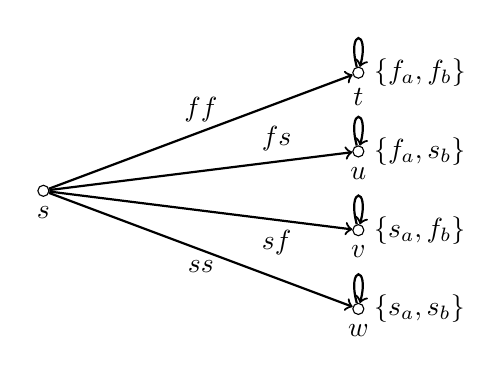
\begin{tikzpicture}
\node(-1) at (2,0) {};
\node[circle,draw=black, minimum size=4pt,inner sep=0pt,  label=below:{$s$}](1) at (0,0) {};
\node[circle,draw=black, minimum size=4pt,inner sep=0pt, , label=below:{$t$}, label = right:{$\{f_a, f_b\}$}](2) at (4,1.5) {};
\node[circle,draw=black, minimum size=4pt,inner sep=0pt, , label=below:{$u$}, label = right:{$\{f_a, s_b\}$}](3) at (4,0.5) {};
\node[circle,draw=black, minimum size=4pt,inner sep=0pt, , label=below:{$v$}, label = right:{$\{s_a, f_b\}$}](4) at (4,-0.5) {};
\node[circle,draw=black, minimum size=4pt,inner sep=0pt, , label=below:{$w$}, label = right:{$\{s_a, s_b\}$}](5) at (4,-1.5) {};

\draw [->,thick](1) to node[above,align=left] {$ff$} (2);
\draw [->,thick](1) to node[above,align=left, near end] {$fs$} (3);
\draw [->,thick](1) to node[below,align=left, near end] {$sf$} (4);
\draw [->,thick](1) to node[below,align=left] {$ss$} (5);
\draw [->,thick] (2) to [loop above]  (2);
\draw [->,thick] (3) to [loop above]  (3);
\draw [->,thick] (4) to [loop above]  (4);
\draw [->,thick] (5) to [loop above]  (5);
\end{tikzpicture}
}
\caption{CGS $\G$ for two agents and two actions. True atomic propositions represented in sets near corresponding states. For readability, self-loops labelled by all combinations of actions, are depicted as unlabelled loops.}
\label{fig::horror}
\end{figure} 
The CGS has five states, $s$, $t$, $u$, $v$, and $w$, and is defined over the set of two actions, $f$ for `folk horror', and $s$ for `sci-fi horror'. Propositional atoms correspond to the outcomes of Anna and Brita's actions with $f_a$ and $s_b$ being true in state $u$ meaning that Anna watches the folk horror film, and Brita watches the sci-fi horror film. 

Now, it is easy to verify that $\G,s \models \varphi$ since Anna can always choose action $f$ and thus let Brita play $f$ as well to reach her own goal. 
\end{example}
\fi

%\begin{example}
  %  Examples of CGSs are presented in Figure \ref{fig::exampleCGM}. In structure $\G_1$ we have two states $s$ and $t$, and the agents can transition between the two states if the execute the same actions. It is easy to verify that $\G_1,s \models \forall x \exists y \assign{x,y} p$ and $\G_1, s \models \forall x \assign{x,x} \lnot p$.
%\end{example}

   \section{Relation to Other Coalition Logics}
\label{sec:expressivity}
In order to appreciate the richness of $\CSL$, we compare the logic to other $\mathsf{CL}$'s. In our comparison we can use two salient features of $\CSL$. First, the logic allows for \textit{arbitrary quantification prefixes for agents' actions}. This includes using the same strategy variable for different agents to capture \textit{strategy sharing}. The second special feature of $\CSL$ is the presence of \textit{explicit action labels} in its syntax.

\begin{definition}[Expressivity]
    Let $\mathsf{L}_1$ and $\mathsf{L}_2$ be two languages, and let $\varphi \in \mathsf{L}_1$ and $\psi \in \mathsf{L}_2$. We call $\varphi$ and $\psi$ \emph{equivalent}, if for any CGS $\G$ and state $s \in \G$: 
    %it holds that 
    $\G,s \models \varphi$ iff $\G, s \models \psi$.  If for all $\varphi \in \mathsf{L}_1$ there exists an equivalent $\psi \in \mathsf{L}_2$, then $\mathsf{L}_2$ is \emph{at least as expressive as } $\mathsf{L}_1$ ($\mathsf{L}_1 \leqslant \mathsf{L}_2$). And $\mathsf{L}_2$ is \emph{strictly more expressive than } $\mathsf{L}_1$ ($\mathsf{L}_1 < \mathsf{L}_2$) if $\mathsf{L}_1 \leqslant \mathsf{L}_2$ and $\mathsf{L}_2 \not \leqslant \mathsf{L}_1$.
\end{definition}

These two features of $\CSL$, arbitrary quantification prefixes and explicit actions, on their own are not unique in the landscape of logics for strategic reasoning. %Thus, 
Arbitrary quantification prefixes are a hallmark feature of the whole family of \textit{strategy logics} (see, e.g., \cite{mogavero10,belardinelli19}), to which $\CSL$ belongs. Indeed, $\CSL$ can be considered as a variation of the next-time fragment of $\mathsf{SL}$. %\textit{strategy logic with simple goals} ($\mathsf{SL[SG]}$) \cite{belardinelli19}, 
%which, in turn, is an extension of $\mathsf{ATL}^\ast$ \cite{alur02} with arbitrary quantification prefixes for agents' strategies. 
The idea to refer to actions in the language has also been explored, with %, perhaps, 
a prime example being $\mathsf{ATL}$ \textit{with explicit strategies} ($\mathsf{ATLES}$) \cite{walther07}. Another example of such a logic %with explicit actions 
is \textit{action logic} %($\mathsf{AL}$) 
\cite{borgo07}.%, which we will deal with later in this section.

Even though both of the main features of $\CSL$ have been explored in the literature, to our knowledge, $\CSL$ is the first logic for strategic reasoning that combines \textit{both} of them. %To further demonstrate the unique position of our logic in the landscape of related logics, we compare it to some known coalition logics. %explored in literature. 


%It is easy to show that $\CSL$ and $\mathsf{ATLES}$ are, expressivity-wise, incomparable. Indeed, in the former we can exploit arbitrary quantification prefix, and in the latter we have additional temporal expressivity. 

 %Moreover, $\CSL$ allows for actions of agents to be explicitly referenced in the logic language. These two features combined, i.e. arbitrary quantification prefixes and explicit action labels, make $\CSL$ quite unique in the landscape of the logics for strategic reasoning. 

 \paragraph{Coalition logic and quantified coalition logic} The original \textit{coalition logic} ($\mathsf{CL}$) \cite{pauly02}, similarly to $\mathsf{ATL}$, allows only single alternation of quantifiers in coalitional modalities. Moreover, this quantification is implicit. Thus, $\mathsf{CL}$ extends the language of propositional logic with constructs $\langle \! \langle C \rangle \! \rangle \varphi$ that mean `there is a strategy for coalition $C$ to achieve $\varphi$ in the next step'. % (whatever agents outside of the coalition do at the same time)'. 
 In \textit{quantified coalition logic} ($\mathsf{QCL}$) \cite{agotnes08}, constructs $\langle \! \langle C \rangle \! \rangle \varphi$ are substituted with $\langle P \rangle \varphi$ meaning `there exists a coalition $C$ satisfying property $P$ such that $C$ can achieve $\varphi$'. Since $\mathsf{QCL}$ is as expressive as $\mathsf{CL}$ (although exponentially more succinct), we will focus only on $\mathsf{CL}$. 
 
 To introduce the semantics of $\mathsf{CL}$, we will denote the choice of actions by coalition $C \subseteq Agt$ with $|Agt| = n$ as $\sigma_C$, and denote $Agt \setminus C$ as $\overline{C}$. Finally, $\sigma_C \cup \sigma_{{\overline{C}}} \in \mathcal{D}$ is a decision. The semantics of $\langle \! \langle C \rangle \! \rangle \varphi$ for a given CGS $\G$ is then defined as 
  \begin{alignat*}{3}
        &\G,s \models \langle \! \langle C \rangle \! \rangle \varphi && \text{ iff } && \exists \sigma_C, \forall \sigma_{\overline{C}} : \G,t \models \varphi \\
        & && &&\text{ with } t \in S \text{ s.t. } \langle s, \sigma_C \cup \sigma_{\overline{C}}, t \rangle \in R.   
\end{alignat*}     
 
The translation from formulas $\mathsf{CL}$ to formulas of $\CSL$ can be done recursively using the following schema for coalitional modalities: 
$tr(\langle \! \langle C \rangle \! \rangle \varphi) \to \exists \vec x \forall \vec y \assign{\vec x, \vec y} tr(\varphi)$, 
where variables $\vec x$ (all different) quantify over actions of $C$, and $\vec y$ (all different) quantify over actions of $Agt \setminus C$. 

At the same time, one cannot refer to particular actions in $\mathsf{CL}$ formulas, as well as express sharing strategies between agents. We can exploit either of these features to show that $\CSL$ is strictly more expressive than $\mathsf{CL}$. 
Indeed, consider a $\CSL$ formula $\exists x \assign{x, x} \lnot p$ meaning that there is an action that \textit{both} agents 1 and 2 should use to reach a $\lnot p$-state. We can construct two CGSs that are indistinguishable by any $\mathsf{CL}$ formulas. At the same time,   $\exists x \assign{x, x} \lnot p$ will hold in one structure and be false in another. 

Consider two structures depicted in Figure \ref{fig::exampleCGM}. 
\begin{figure}[h!]
\centering
\scalebox{0.7}{
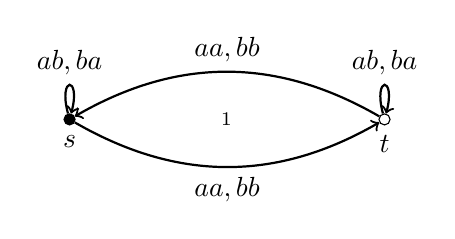
\begin{tikzpicture}
\node(-1) at (2,0) {$\G_1$};
\node[circle,draw=black, minimum size=4pt,inner sep=0pt, fill = black, label=below:{$s$}](1) at (0,0) {};
\node[circle,draw=black, minimum size=4pt,inner sep=0pt, , label=below:{$t$}](2) at (4,0) {};

\draw [->,thick](1) to [loop above] node[above, align=left] {$ab, ba$} (1);
\draw [->,thick](1) to [bend right] node[below,align=left] {$aa, bb$} (2);
\draw [->,thick] (2) to [bend right] node[above,align=left] {$aa, bb$} (1);
\draw [->,thick] (2) to [loop above] node[above,align=left] {$ab, ba$} (2);
\end{tikzpicture}
\hspace{6mm}
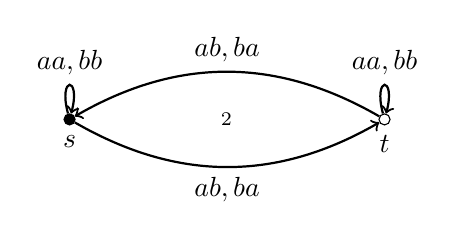
\begin{tikzpicture}
\node(-1) at (2,0) {$\G_2$};
\node[circle,draw=black, minimum size=4pt,inner sep=0pt, fill = black, label=below:{$s$}](1) at (0,0) {};
\node[circle,draw=black, minimum size=4pt,inner sep=0pt, , label=below:{$t$}](2) at (4,0) {};

\draw [->,thick] (1) to [loop above] node[above, align=left] {$aa, bb$} (1);
\draw [->,thick](1) to [bend right] node[below,align=left] {$ab, ba$} (2);
\draw [->,thick] (2) to [bend right] node[above,align=left] {$ab, ba$} (1);
\draw [->,thick] (2) to [loop above] node[above,align=left] {$aa, bb$} (2);
\end{tikzpicture}
}
\caption{CGSs $\G_1$ and $\G_2$ for two agents and two actions. Propositional variable $p$ is true in black states.}
\label{fig::exampleCGM}
\end{figure} 
It is easy to see that $\G_1,s$ and $\G_2,s$ cannot be distinguished by any $\mathsf{CL}$ formula\footnote{These structures are, in fact, in the relation of \textit{alternating bisimulation} \cite{agotnes07}, and hence satisfy the same formulas of $\mathsf{CL}$ and $\mathsf{ATL}$. The discussion of bisimulations for all the logics we mention is, however, beyond the scope of this paper, and we leave it for future work.}. Indeed, both structures agree on the valuation of propositional variable $p$ in corresponding states. Moreover, none of the agents, 1 and 2, can on their own force a transition from state $s$ to state $t$. At the same time, the grand coalition $\{1,2\}$ can match any transition in one structure with a transition with the same effect in the other structure. %force any transition in both structures. 
Now, we can verify that $\G_1,s \models \exists x \assign{x, x} \lnot p$ and $\G_2,s \not \models \exists x \assign{x, x} \lnot p$. For the case of  $\G_1,s \models \exists x \assign{x, x} \lnot p$, it is enough to assign action $a$ to $x$ to have $\G_1,s \models \assign{a, a} \lnot p$. To make $\exists x \assign{x, x} \lnot p$ hold in $\G_2, s$, one needs to provide an action that once executed by both agents will force the transition to state $t$. It is easy to see that there is no such an action in $\G_2,s$.

Having the translation from $\mathsf{CL}$ to $\CSL$ on the one hand, and the indistinguishability result on the other, we hence conclude that $\CSL$ is \textit{strictly more expressive} than $\mathsf{CL}$.

\begin{proposition}
\label{prop:cslVScl}
    $\mathsf{CL} < \CSL$.
\end{proposition}

\paragraph{Conditional strategic reasoning and socially friendly $\mathsf{CL}$} With the expressive power of $\CSL$ we can go much further than the classic $\mathsf{CL}$. In particular, we can express in our logic such interesting $\mathsf{CL}$'s like \textit{logic for conditional strategic reasoning} ($\mathsf{ConStR}$) \cite{goranko22}, \textit{socially friendly $\mathsf{CL}$} ($\mathsf{SFCL}$) \cite{goranko18}, and \textit{group protecting $\mathsf{CL}$} ($\mathsf{GPCL}$)  \cite{goranko18}. 

Presenting the semantics of the aforementioned logic is beyond the scope of this paper. However, we would like to point out that all of the logics can be captured by \textit{basic strategy logic} ($\mathsf{BSL}$) \cite{goranko23}, a variant of $\mathsf{SL}$, where each agent has her own associated strategy variable. Differently from $\CSL$, $\BSL$ allows for all standard temporal modalities like `ne\textsf{X}t', `\textsf{U}ntil' and `\textsf{G}lobally'. At the same time, $\BSL$ does not allow for variable sharing and does not explicitly refer to actions or strategies. Moreover, it is conjectured that $\BSL$ does not have a recursive axiomatisation, while $\CSL$ has a finitary complete axiomatisation (see Section \ref{sec:axiom}).

Translations of all coalition logics introduced in this paragraph into formulas of $\mathsf{BSL}$ are presented in \cite{goranko23}, where it is also claimed that $\mathsf{BSL}$ is strictly more expressive than all the aforementioned logics. The translation does not employ any temporal features of $\mathsf{BSL}$ apart from `ne\textsf{X}t', and thus the same translation also works for $\CSL$. Moreover, we can use either strategy sharing or explicit actions to argue that $\CSL$ is strictly more expressive than the considered coalition logics. As an example, an argument for the case of $\mathsf{SFCL}$ is given in \cite{csl}. %the Appendix.

%For the sake of an example, 


\begin{proposition}
    $\mathsf{ConStR} < \CSL$, $\mathsf{SFCL} < \CSL$, $\mathsf{GPCL} < \CSL$.
\end{proposition}

\paragraph{Action logic} 

A perhaps most relevant to $\CSL$ coalition logic in the literature is \textit{action logic} ($\mathsf{AL}$) \cite{borgo07}, which is a fragment of \textit{multi-agent PDL with quantificaiton} ($\mathsf{mPDLQ}$) \cite{borgo05}. $\mathsf{AL}$ extends the language of propositional logic with so-called \textit{modality markers} $[M]$, which are, essentially, prefixes of size $|Agt| = n$, each element of which can either be a quantifier $Q_i x_i$ with $Q_i \in \{\forall, \exists\}$ or an explicit action \cite{borgo05,borgo05b}. An important feature here is that \textit{there are no repeating variables in modality markers}. Finally, to the best of our knowledge, there is no axiomatisation of  $\mathsf{AL}$.

Given a modality marker $[M]$, we denote by $\sigma_\exists$ a choice by all the existentially quantified agents, by $\sigma_\forall$ a choice by all the universally quantified agents, and by $\sigma_{act}$ explicit actions in the corresponding positions in $[M]$. Then modality markers have the following semantics:
  \begin{alignat*}{3}
        &\G,s \models [M] \varphi && \text{ iff } && \exists \sigma_\exists, \forall \sigma_\forall : \G,t \models \varphi \\
        & && &&\text{ with } t \in S \text{ s.t. } \langle s, \sigma_\exists \cup \sigma_\forall \cup \sigma_{act}, t \rangle \in R.   
\end{alignat*}   
\iffalse
\begin{gather*}
    \G,s \models [M] \varphi \text{ iff }\\
    \text{ for all } x_1, ...., x_m \text{ with } \exists x_i \in M, \exists a_i \in \Ac \text{ s.t. } \\
        \langle s, A, s'\rangle \in R \text{ and } \G,s'\models \varphi, \text{ for all } A \text{ s.t. } a_1, ..., a_m \sqsubseteq A.  
\end{gather*}
\fi
\iffalse
  \begin{alignat*}{3}
        &\G,s \models [M] \varphi && \text{ iff } && \text{ for all } x_1, ...., x_m \text{ with } \exists x_i \in M, \exists a_i \in \Ac \text{ s.t. }\\
        & && &&\langle s, A, s'\rangle \in R \text{ and } \G,s'\models \varphi,\\ & && &&\text{ for all } A \text{ s.t. } a_1, ..., a_m \sqsubseteq A.  
\end{alignat*}    
\fi
Intuitively, $\G,s \models [M] \varphi$ holds if and only if there is an assignment of actions to all existentially quantified variables in modality marker $M$ such that no matter which actions are assigned to the universally quantified variables, once combined with the explicit actions, the outcome state satisfies $\varphi$. This is in line with the semantics of $\mathsf{CL}$ as we basically choose actions for a coalition (existentially quantified variables) and verify $\psi$ in all possible outcomes given this choice. 

Formulae $[M]\varphi$ of $\mathsf{AL}$ can be translated into formulae of $\CSL$ of the form $\exists \vec x \forall \vec y \assign{t_1, ..., t_n} \varphi$, where $\vec x$ and $\vec y$ with $|\vec x| + |\vec y| \leqslant n$ are possibly empty sequences of variables for the existentially and universally quantified agents respectively, $t_i := x_i$ if there is a quantifier in position $i$ in the modality marker, and $t_i:= a_i$ if there is action $a_i$ in the $i$th posiiton in the modality marker. Also recall that $\mathsf{AL}$ does not allow for sharing strategies (while $\CSL$ does), i.e. all $x_1, ..., x_m$ in the modality marker are unique. 

To show that $\CSL$ is more expressive than $\mathsf{AL}$, we need the following proposition. Its proof utilises the strategy sharing feature of $\CSL$ and can be found in \cite{csl}. %the Appendix. %approach the relative expressivity of $\CSL$ and $\mathsf{AL}$ formally, we prove the following lemma. 

\begin{proposition}
\label{lemma:exp}
    $\mathsf{AL}$ is not at least as expressive as $\CSL$.
\end{proposition}
\iffalse
\begin{proof}
    Consider $\exists x \assign{x, x} \lnot p \in \CSL$, and assume towards a contradiction that there is an equivalent $\varphi \in \mathsf{AL}$. Since we have a countably infinite set of constants $\mathcal{C}$ (and hence actions) at our disposal  and due to the fact that $\varphi$ is finite, we can assume that there are actions $a$ and $b$ that do not appear explicitly in $\varphi$. 

Now, consider two concurrent game structures defined over two agents and two actions in Figure \ref{fig::exampleCGM}. As we have already seen in our argument for Proposition \ref{prop:cslVScl}, $\G_1,s \models \exists x \assign{x, x} \lnot p$ and $\G_2,s \not \models \exists x \assign{x, x} \lnot p$. What is left to show is that $\varphi$ cannot distinguish the two structures, i.e. $\G_1,s \models \varphi$ if and only if $\G_2, s \models \varphi$. The proof is by induction on the complexity of $\varphi$, and the details can be found in \cite{csl}. %the Appendix.
\end{proof}
\fi

Having the translation from $\mathsf{AL}$ to $\CSL$ on the one hand, and Lemma \ref{lemma:exp} on the other, we can conclude that $\CSL$ is strictly more expressive than $\mathsf{AL}$.

\begin{corollary}
\label{alVScsl}
    $\mathsf{AL} < \CSL$.
\end{corollary}



\paragraph{The expressivity landscape}
In this section we have explored the relationship between $\CSL$ and other notable $\mathsf{CL}$'s from the literature. The overall expressivity landscape of the considered logics is presented in Figure \ref{fig:expressivity}.

\begin{figure}[h!]
\centering
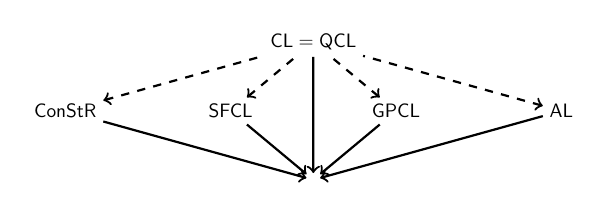
\begin{tikzpicture}[scale=0.7, transform shape]
\node (constr) at (0,0) {$\mathsf{ConStR}$};
\node (sfcl) at (3,0) {$\mathsf{SFCL}$};
\node (gpcl) at (6,0) {$\mathsf{GPCL}$};
\node (al) at (9,0) {$\mathsf{AL}$};
\node (csl) at (4.5,-1.25) {$\CSL$};
\node (cl) at (4.5,1.25) {$\mathsf{CL} = \mathsf{QCL}$};

\draw[thick, dashed, <-] (constr) to  (cl);
\draw[thick, dashed, <-] (sfcl) to (cl);
\draw[thick,dashed, <-] (gpcl) to (cl);
\draw[thick, dashed, <-] (al) to (cl);
\draw[thick,<-] (csl) to (cl);
\draw[thick,<-] (csl) to (constr);
\draw[thick,<-] (csl) to (sfcl);
\draw[thick,<-] (csl) to (gpcl);
\draw[thick,<-] (csl) to (al);
\end{tikzpicture}
\caption{Overview of the expressivity results. An arrow from $\mathsf{L}_1$ to $\mathsf{L}_2$ means $\mathsf{L}_1 <\mathsf{L}_2$. Dashed arrows represent results from the literature. Solid arrows are new results.}
\label{fig:expressivity}
\end{figure}






\section{Proof Theory}
\label{sec:axiom}

%\subsection{Context}
Perhaps the best-known results in the field are complete axiomatisations of $\mathsf{CL}$ \cite{pauly02,goranko13} and $\mathsf{ATL}$ \cite{goranko06} (see \cite{walther06,goranko09} for more constructive approaches). Other completeness results include axiomatisations for logics based on $\mathsf{CL}$ and $\mathsf{ATL}$, like already mentioned $\mathsf{SFCL}$ \cite{goranko18}, $\mathsf{ATLES}$ \cite{walther07}, as well as \textit{epistemic} $\mathsf{CL}$ \cite{agotnes19}, \textit{resource-bounded} $\mathsf{CL}$ \cite{alechina11} and $\mathsf{ATL}$ \cite{nguyen18}, and $\mathsf{ATL}$ \textit{with finitely bounded semantics} \cite{goranko19}, to name a few.

In the context of strategy logics, we have quite an opposite picture. Since the inception of $\mathsf{SL}$ \cite{mogavero10}, its axiomatisation has been an open problem. The same can be said about any of the fragments of $\mathsf{SL}$. %, like \textit{one-goal} $\mathsf{SL}$ ($\mathsf{SL[1G]}$). %Indeed, the satisfiability problem for the original $\mathsf{SL}$ is $\Sigma^1_1$-hard \cite{mogavero16}, which implies that $\mathsf{SL}$ is not recursively axiomatisable. This does not rule out, though, the existentence of an \textit{infinitary} axiomatisation.
%A fragment of $\mathsf{SL}$, called \textit{one-goal} $\mathsf{SL}$ ($\mathsf{SL[1G]}$), has a decidable satisfiability problem so there is a hope of having a proof system for it. However, $\mathsf{SL[1G]}$ subsumes $\mathsf{ATL}^\ast$, and providing a complete axiomatisation of the latter is yet another long-standing open problem. 
The lack of axiomatisations of \textit{any} (fragment of) $\mathsf{SL}$ can be traced back to the two main features of the logic: quantification over strategies and arbitrary quantification prefixes. %To understand these nuances of $\mathsf{SL}$ better, we need the following defintion.

%\begin{definition}
%    Let $\G = \tuple{n,\Ac, \mathcal{D}, S,R, \mathcal{V} }$ be a CGS. A \emph{(memoryless) strategy} for an agent $i \in n$ is a function $\sigma_i: S \to \Ac$. The set of all strategies of all agents is denoted as $\Sigma (\G)$. An \emph{assignment} is a function $\chi: \V \cup n \to \Sigma (\G)$ that assigns strategies from $\Sigma (\G)$ to each agent and each variable.
%\end{definition}

%The language of $\mathsf{SL}$ extends the language of \textit{linear temporal logic} ($\mathsf{LTL})$ with constructs for quantification over strategies $\exists x \varphi$ and for binding agents to strategies $(x,i) \varphi$. The latter means `agent $i$ can achieve $\varphi$ by using strategy assigned to $x$'. The semantics of $\mathsf{SL}$ is defined relative to a given assignment $\chi$:
   % \begin{alignat*}{3}
     %   &\G,s\models_\chi \exists x \varphi &&\text{ iff } &&\exists \sigma_i \text{ for all agents } i \text{ bound to } x: \G,s\models_{\chi_{\sigma_i}^x} \varphi\\
     %   &\G,s\models_\chi (x,i) \varphi &&\text{ iff } && \G,s\models_{\chi_{\chi(x)}^i} \varphi
    %\end{alignat*}
%In the semantics, $\chi_{\sigma_i}^x$ stands for a variant of $\chi$ such that variable $x$ is assigned strategy $\sigma_i$ (and everything else is the same), and $\chi_{\chi(x)}^i$ stands for a variant  of $\chi$, where agent $i$ is assigned the strategy associated with variable $x$ (and everything else is the same).

%Having these definitions in mind, it is easy to note that, firstly, the quantification prefix of $\mathsf{SL}$ formulas can be arbitrary. 
Indeed, arbitrary alternation of quantifiers in $\mathsf{SL}$ is quite different from the fixed quantification prefix of $\mathsf{CL}$ and $\mathsf{ATL}$ that allow only prefixes $\exists \forall$ and $\forall \exists$. Secondly, quantification over strategies\footnote{A \emph{(memoryless) strategy} for an agent $i \in n$ is a function $\sigma_i: S \to \Ac$.}  in $\mathsf{SL}$ is essentially a second-order quantification over functions. We believe that these two features combined are the root cause of the fact that no complete axiomatisations of (fragments of) $\mathsf{SL}$ %or its fragments 
have been proposed so far. 

In $\CSL$ we focus on arbitrary quantification prefixes. To solve this sub-problem, we consider only ne$\mathsf{X}$t-time modalities $\assign{t_1\cdots t_n} \varphi$ and deal with the immediate outcomes of agents' choices. 
%Other temporal modalities, like $\mathsf{U}$ntil and $\mathsf{E}$ventually would require a more complicated construction as their truth values depend on the whole computation paths rather than just the next step (see \cite{goranko06} on how to deal with them in the context of $\mathsf{ATL}$). 
This allows us, in particular, to consider quantification over actions rather than strategies. %(see the semantics of $\CSL$ and $\mathsf{SL}$ for comparison). 
Hence, quantification in $\CSL$ is a first-order quantification, instead of the second-order quantification of $\mathsf{SL}$. %The relation between various fragments of $\mathsf{SL}$ and the corresponding induced fragments of $\mathsf{FOL}$ is explored in \cite{mogavero15}.

In our proof, we take as inspiration the completeness proof for \textit{first-order modal logic} ($\mathsf{FOML}$) with constant domains \cite{Garson1984}. Our construction is quite different, though, as in $\mathsf{FOML}$ variables appear in $n$-ary predicates, and in $\CSL$ variables are placeholders for transition labels.  

\subsection{Axiomatisation of $\CSL$}

\begin{definition}[Axiomatisation]
    The \emph{axiom system} for $\CSL$ consists of the following axiom schemata and rules, where $\vec{t}=t_1,\ldots,t_n$ for $n\geqslant 1$, and $t$ and each $t_i$ are either a variable or a constant. %, and likewise for $t$.
    $$
    %\small
\begin{array}{c
%@{\qquad}
l}

    \mathsf{PC}  & \text{Every propositional tautology}  
  \\
     \mathsf{K} & ( \assign{\vec{t}} \varphi \land \assign{\vec{t}}\psi) \leftrightarrow \assign{\vec{t}}(\varphi \land \psi )
   \\
   \mathsf{\mathsf{N} } & \neg \assign{\Vec{t}}\varphi \leftrightarrow \assign{\vec{t }}\neg \varphi 

   \\
   \mathsf{E} & \forall x \varphi \to \varphi[t/x]
\\
\mathsf{B} & \forall x \assign{\vec t} \varphi \imp \assign{\vec t} \forall x \varphi, \text{s.t. } t_i \neq x \text{ for all } t_i %\text{, where each } t_i \text{ is different from $x$} %\qquad   % x\neq t_i \text{ for all $i\leq n$} 
\\
\mathsf{MP} & \text{From } \varphi, \varphi \to \psi, \text{ infer } \psi
\\
\mathsf{Nec} & \text{From } \varphi, \text{ infer } \assign{\vec t }\varphi
\\
\mathsf{Gen} & \text{From } \varphi\to \psi[t/x] , \text{ infer } \varphi\to \forall x \psi, \text{ if $t \not \in \varphi$} %\text{ if $t$  does not appear in $\varphi$}
\end{array}
$$
\iffalse
\begin{tabular}{p{0.33\textwidth} p{0.33\textwidth} p{0.33\textwidth}}

   \begin{prooftree}
       \AxiomC{$\varphi$}\LeftLabel{$\mathsf{MP}$}
       \AxiomC{$\varphi \to \psi$}
       \BinaryInfC{$\psi$}
   \end{prooftree} 
   &  
  \begin{prooftree}
       \AxiomC{$\varphi$}\LeftLabel{$\mathsf{Nec}$}
         \UnaryInfC{$\assign{\vec t }\varphi $}
   \end{prooftree} 
   
     &  \begin{prooftree}
       \AxiomC{$\varphi\to \psi $}\RightLabel{$x\notin \FV(\varphi  )$}\LeftLabel{$\mathsf{Gen}$}
        \UnaryInfC{$\varphi\to \forall x \psi$}
   \end{prooftree} 

     
\end{tabular}
\fi
\noindent An axiomatic derivation $\pi$ is a finite sequence of formulae $\varphi_1,\ldots, \varphi_m$ where for each $i\leqslant m$:  either $\varphi_i$ is an instance of one of the axiom schemata of $\CSL$, or it is obtained from some preceding formulae in the sequence using rules $\mathsf{MP}$, $\mathsf{Nec}$, or $\mathsf{Gen}$.
We write   $\vdash\varphi$ and say that  $\varphi$ is \emph{$\CSL$ derivable} (or simply derivable)  iff there is a derivation $\pi$ whose last element is $\varphi$. Given a set of formulae $X$, we write $X \vdash \varphi$ iff there is a finite subset $Y $ of $X$ such that %$\vdash_\CSL \bigwedge Y \imp \varphi$. 
$\vdash \bigwedge Y \imp \varphi$.
\end{definition}


We will freely use the following proposition in the rest of the paper. Its proof is standard, and we omit it for brevity. 

\begin{proposition}\label{prop.first}
    The following formulae are $\CSL$ derivable, where $\vec{t}=t_1,\ldots,t_n$, and each $t_i$ is either a constant or a variable: 
    \begin{enumerate}
        \item $\assign{\vec{t}}(\varphi\imp \psi)\imp (\assign{\vec{t}}\varphi) \imp (\assign{\vec{t}}\psi); $
        \item $\forall x (\varphi \imp \psi)\imp (\varphi \imp \forall x \psi)$ with $x\notin \FV(\varphi);$
        \item $\exists z (\varphi \imp \forall y \varphi )$ with $z\notin \FV(\forall y \varphi).$
      \end{enumerate}
      Moreover, if $\varphi\imp \psi$ is derivable, so is $\assign{\vec{t}}\varphi \imp \assign{\vec{t}} \psi $.
\end{proposition}


\begin{lemma}\label{lemma:sound}
    Each axiom schema of $\CSL$ is valid and each rule of $\CSL$ preserves validity.%: if the premised of a rule are valid so it is its conclusion. 
\end{lemma}

The proof of Lemma \ref{lemma:sound} is done by the application of the definition of the semantics, and it can found in \cite{csl}. %the Appendix.

\iffalse
\begin{proof}
 For the sake of simplicity, we only consider closed instances of the axiom schemata. Validity of other axiom schemata and the soundness of the rules of inference can be shown similarly.
 
 ($\mathsf{N}$). Suppose that $\G,s\models \neg \assign{\vec{{a}}}\varphi$. By the definition of the semantics, this means that $\G,s\not \models \assign{\vec{{a}}} \varphi$, i.e. for each   $t\in S$ if   $\tuple{s,\vec{a},t}\in R$,  then we have that $\G,t\not\models \varphi$. From the seriality and functionality of $R$, we can conclude that there is exactly one such $t$, and thus $\G,s\models \assign{\vec{{a}}}\neg \varphi $. For the converse direction, suppose that $\G,s\models \assign{\vec{{a}}}\neg \varphi$. This means that there is a $t$ such that $\tuple{s,\vec{a},t}\in R$ and $\G,t\not\models \varphi$. By functionality of $R$ there is no other $t$ related to $s$ by means of $\vec{a}$, and thus we can conclude that $\G,s\models \neg \assign{\vec{{a}}}\varphi$. 

 ($\mathsf{B}$). Assume that $\G,s \models \forall x \assign{\vec t} \varphi$, where $x$ is different from every $t_i$. Since the formula is closed, this is just $\G,s \models \forall x \assign{\vec{ {a}}} \varphi$ for some $\vec{a}\in \mathcal D$. By the truth definition, this is equivalent to $\G,s \models \assign{\vec{{a}}} (\varphi [{b}/x])$ for every $b\in \Ac$, which means $\G,s\models \assign{\vec{ a}} \forall x \varphi $.
%\begin{description}
 %   \item[($\mathsf{N}$)] Suppose that $\G,s\models \neg \assign{\vec{{a}}}\varphi$. By the definition of the semantics, this means that $\G,s\not \models \assign{\vec{{a}}} \varphi$, i.e. for each   $t\in S$ if   $\tuple{s,\vec{a},t}\in R$,  then we have that $\G,t\not\models \varphi$. From the seriality and functionality of $R$, we can conclude that there is exactly one such $t$, and thus $\G,s\models \assign{\vec{{a}}}\neg \varphi $. For the converse direction, suppose that $\G,s\models \assign{\vec{{a}}}\neg \varphi$, this means that there is an $t$ such that $\tuple{s,\vec{a},t}\in R$ and $\G,t\not\models \varphi$. By functionality of $R$ there is no other $t$ related to $s$ by means of $\vec{a}$, and thus we can conclude that $\G,s\models \neg \assign{\vec{{a}}}\varphi$. 
  %  \item[($\mathsf{B}$)] Assume that $\G,s \models \forall x \assign{\vec t} \varphi$, where $x$ is different from every $t_i$. Since the formula is closed, this is just $\G,s \models \forall x \assign{\vec{ {a}}} \varphi$ for some $\vec{a}\in \mathcal D$. By the truth definition, this is equivalent to $\G,s \models \assign{\vec{{a}}} (\varphi [{b}/x])$ for every $b\in \Ac$, which means $\G,s\models \assign{\vec{ a}} \forall x \varphi $. \qedhere 
%\end{description}
\end{proof}
\fi



Our completeness proof is based on the canonical model construction, where states are maximal consistent sets with the $\forall$-property.

\begin{definition}[Maximal Consistent Sets]
Let $Z$ be a set of $\CSL$ sentences over a given signature and $X\subseteq Z$. We say that: (i)$X$ is \emph{consistent} iff $X\not\vdash \bot$, (ii) $X$ is \emph{maximally consistent} (MCS) iff it is consistent and there is no other consistent set of sentences $Y\subseteq Z$ s.t. $X\subset Y$, %that strictly includes $X$ 
and (iii) $X$ has the \emph{$\forall$-property} iff for every formula $\varphi$ over the same signature as $Y$  and variable $x$, there is a constant $a$ such that $\varphi[a/x]\to \forall x \varphi\in X$, where $\varphi[a/x]$ is closed. We will call a set satisfying all the three requirements $\forall$-MCS.

\end{definition}


Let $\alpha=\tuple{n,\mathcal{C},\Ap}$ be a signature. We denote by $\alpha^\star$ the signature $\tuple{n,\mathcal{C}\cup \mathcal{C}^\star,\Ap}$ where $\mathcal{C}^\star$ is countably infinite, and $\mathcal{C}\cap \mathcal{C}^\star = \emptyset$. 

Next lemma shows  that each consistent set of sentences over a given signature $\alpha$  can be extended to a consistent set of sentences over $\alpha^\star$ having the $\forall$-property.  Its proof follows the standard technique in $\mathsf{FOML}$ \cite{Cresswell1996-CREANI-3}, and can be found in \cite{csl}. %the Appendix. %we report it here for the sake of completeness. 


\begin{lemma}\label{lemma:expConst}
    If $X$ is a consistent set of sentences over a given signature $\alpha$, then there is a consistent set of sentences $Y$ over $\alpha^\star$ such that $X\subseteq Y$, and $Y$ has the $\forall$-property.  
\end{lemma}
\iffalse
\begin{proof}
    Let $E$ be an enumeration of sentences of the form $\forall x \varphi$ over $\alpha^\star$. We define a sequence of sets of sentences $Y_0,Y_1,\ldots$ with $Y_0=X$ and $Y_{n+1}=Y_n \cup \set{ \varphi[a/x]\to \forall x \varphi}$ where $\forall x \varphi$ is the $n+1$-th sentence in $E$, and $a$ is the first constant in the enumeration occurring neither in $Y_n$ nor in $\varphi$. Since $Y_0$ is over $\alpha$, $Y_n$ is obtained by the addition of $n$ sentences over $\alpha^\star$, and $\alpha^\star$ includes a countably infinite set of new constants, we can always find such an $a$. 
    
    Now we show that $Y_{n+1}$ constructed in the described way is consistent. For this, assume towards a contradiction that $Y_n$ is consistent and $Y_{n+1}$ is not. This means that there is a finite set of sentences $U\subseteq Y_n$ such that $U\cup \set{\varphi [a/x]\to \forall x \varphi}\vdash \bot$. By the rules of $\CSL$ we thus obtain that (i) $U\vdash \varphi [a/x]$ and (ii) $U\vdash \neg \forall x \varphi$. Since $a$ does not appear in $Y_n$, we can use the  $\mathsf{Gen}$ rule of inference and conclude that $U\vdash \forall x \varphi$. In conjunction with (ii) this amounts to the fact that $Y_n$ is not consistent, and hence we arrive at a contradiction.
    %and thus, because of (ii), that $U\vdash \bot$ which contradicts that $Y_n$ is consistent. 
    
    Define $Y$ as $\bigcup_{n\in \mathbb{N} }Y_n$. It is now easy to see that $Y$ is consistent and has the $\forall$-property. 
\end{proof}
\fi

The proof of the following lemma (Lindenbaum Lemma) is standard, and we omit it for brevity.


\begin{lemma}
\label{lemma:mcs}
Let $X$ be a consistent set of sentences 
over a given signature, then there is %a maximal consistent set of sentences 
an MCS $Y$ over the same signature such that $X\subseteq Y$.
\end{lemma}

The next two lemmas will be instrumental in the proof of the Truth Lemma, and showing that the canonical model we are to define in this proof is indeed a CGS. 


\begin{lemma}\label{lemma:diamond}
Let $X$ be a consistent set of sentences over a given signature and let $\vec{a}$ be a tuple of constants,   
 then the set $Y_{\vec{a}}=\set{\psi\mid \assign{\vec{a}}\psi\in X}$ is also consistent.
\end{lemma}
\begin{proof}
If $Y_{\vec{a}}$ is empty, the result is trivially valid. Assume that $\varphi \in Y_{\vec{a}}$ and  suppose
    towards a contradiction, that set $Y_{\vec{a}}$ is not consistent. This implies that $(\psi_1\land \cdots \land \psi_m)\to \neg \varphi$ for some finitelty many $\psi_1,\ldots, \psi_m$ in $Y_{\vec{a}}$. Using Proposition \ref{prop.first}(1) and propositional reasoning, we can then derive $\assign{\vec{a}}\psi_1 \land \cdots \land \assign{\vec a}\psi_m\imp \assign{\vec a} \neg \varphi  $. Since $\assign{\vec{a}}\psi_i\in X$, we conclude by $\mathsf{MP}$ that $X \vdash \assign{\vec a} \neg \varphi$. Then, by $\mathsf{N}$ and $\mathsf{MP}$  we can further derive $X\vdash \neg \assign{\vec{a}}\varphi$, which contradicts $\assign{\vec a} \varphi\in X$. 
\end{proof}



%The following  lemma will be used to show that the canonical model is a CGS and in the proof of the truth lemma to follow. 

\begin{lemma}
\label{lemma:lindy}
%Let $X$ be a maximal consistent set of sentences with the $\forall$-property over a given signature containing infinitely many constants. Then there exists a consistent set of sentences $Y$ over the same signature that has the $\forall$-property and such that $Z=\set{\psi \mid \assign{\vec{a}} \psi \in X} \subseteq Y$.
Let $X$ be a $\forall$-MCS over a given signature containing infinitely many constants. Then there exists a $\forall$-MCS $Y$ over the same signature such that $Z=\set{\psi \mid \assign{\vec{a}} \psi \in X} \subseteq Y$.
\end{lemma}
\begin{proof}
If $Z = \emptyset$, the lemma trivially holds. %there is nothing to prove. 
So assume $\varphi \in Z$, and let $E$ be an enumeration of all sentences of the form $\forall x \xi$, and $C$ an enumeration of the constants in the given signature. We define a sequence of sentences $\theta_0, \theta_1, \ldots$ where $\theta_0 = \varphi$, and given $\theta_n$, we set $\theta_{n+1} = \theta_n \land (\xi[a/x] \imp \forall x \xi)$, where $\forall x \xi$ is the $(n+1)$-th formula in $E$, and $a$ is the first constant in $C$ such that $$(\star)\quad Z \cup \set{\theta_n \land (\xi[a/x] \imp \forall x \xi)} \text{ is consistent.}$$

Let $Y = Z \cup \set{\theta_n \mid n \in \mathbb{N}}$. Clearly $Y$ has the $\forall$-property, and it is consistent if $Z \cup \set{\theta_n}$ is consistent for every $n \in \mathbb{N}$. To show this, we prove that if $Z \cup \set{\theta_n}$ is consistent, then there always exists a constant $a$ satisfying $(\star)$. The set $Z \cup \set{\theta_0} = Z$ is consistent by Lemma \ref{lemma:diamond}. %, this suffices to conclude the proof.

Suppose, towards a contradiction, that $Z \cup \set{\theta_n}$ is consistent but for every constant $a$, the set $Z \cup \set{\theta_n \land (\xi[a/x] \imp \forall x \xi)}$ is inconsistent. Then for each constant $a$, there exist finitely many formulas $\psi_1^a, \ldots, \psi_m^a$ in $Z$ such that $(\psi_1^a \land \cdots \land \psi_m^a) \imp (\theta_n \imp \neg(\xi[a/x] \imp \forall x \xi))$ is derivable. From this, by the rules of $\CSL$, it follows that $(\assign{\vec{a}} \psi_1^a \land \cdots \land \assign{\vec{a}} \psi_m^a) \imp \assign{\vec{a}}(\theta_n \imp \neg(\xi[a/x] \imp \forall x \xi))$ is derivable. Since $\psi_i^a \in Z$ implies $\assign{\vec{a}} \psi_i^a \in X$, we conclude that (i) $\assign{\vec{a}}(\theta_n \imp \neg(\xi[a/x] \imp \forall x \xi)) \in X$ for every constant $a$.

Let $z$ be a variable that occurs neither in $\theta_n$ nor in $\xi$. Consider the sentence $\forall z\, \assign{\vec{a}}(\theta_n \imp \neg(\xi[z/x] \imp \forall x \xi))$. From the $\forall$-property of $X$ and (i), it follows that $\forall z\, \assign{\vec{a}}(\theta_n \imp \neg(\xi[z/x] \imp \forall x \xi)) \in X$. By axiom $\mathsf{B}$, this implies $\assign{\vec{a}} \forall z (\theta_n \imp \neg(\xi[z/x] \imp \forall x \xi)) \in X$, and thus, by (2) of Prop. \ref{prop.first}, we have (ii) $\assign{\vec{a}}(\theta_n \imp \forall z \neg(\xi[z/x] \imp \forall x \xi)) \in X$. Since $\exists z (\xi[z/x] \imp \forall x \xi)$ is derivable in $\CSL$, applying rule $\mathsf{Nec}$ gives $\assign{\vec{a}} \exists z (\xi[z/x] \imp \forall x \xi) \in X$. From this, together with (ii), and using Proposition \ref{prop.first}, %and contraposition, 
we conclude $\assign{\vec{a}} \neg \theta_n \in X$. By the construction of $Z$, this implies $\neg \theta_n \in Z$, which contradicts the assumption that $Z \cup \set{\theta_n}$ is consistent.
\end{proof}



%\begin{lemma}
 %   Let $X$ be any consistent set of formulas that are constructed over a set $Ac$ of actions. There is a set $Y$ of formulas such that 
%\end{lemma}

%\begin{lemma}
%Let $\Gamma$ be a consistent set of formulas of $\CSL$. Then there is a consistent set $\Delta$ of formulas of $\CSL^+$ such that $\Delta$ has the $\forall$-property and $\Gamma \subseteq \Delta$, and where $\CSL^+$ is the extension of $\CSL$ with a new countably infinite set of variables. 
%\end{lemma}

%Hi!

%Next, we need to show that if some formula $\assign{\Vec{t}} \varphi \not \in \Gamma$, then there is a witness set $\Delta$ such that $\lnot \varphi \in \Delta$.

%begin{lemma}
%Let $\Gamma$ be an MCS$^\forall$, and $\assign{\Vec{t}} \varphi \not \in \Gamma$, where $\Vec{t}$ contains only constants. Then there exists an MCS$^\forall$ $\Delta$ over $\CSL^+$ such that $\assign{\Vec{t}} \Gamma \cup \{\lnot \varphi\} \subseteq \Delta$.
%\end{lemma}

%\begin{proof}
    
%\end{proof}


\begin{definition}[Canonical Model]
\label{def:can_model}
Given a signature $\alpha=\tuple{n,\mathcal{C}, \Ap}$, 
the canonical model over $\alpha$ is the tuple $\G^C=\tuple{n, \Ac^C,\mathcal{D}^C, S^C, R^C,$    $\mathcal{V}^C}$, where: 

\begin{itemize}
    %\item each member of $S^C$ is a maximally consistent set of sentences over $\alpha^\star$ having the $\forall$-property; 
    %\item the set $\Ac^C$ is just $\mathcal{C}\cup \mathcal{C}^\star$;
    \item $\Ac^C=\mathcal{C}\cup \mathcal{C}^\star$;
   
    %\item $\mathcal{D}^C$ is ${Ac^C}^n $;
    \item $\mathcal{D}^C = {Ac^C}^n $;
%     \item $S^C = \{X \mid X \text{ is a maximally consistent set of sentences}$ $\text{ over }$ $\alpha^\star \text{ with the } \forall\text{-property}\}$;
 \item $S^C = \{X \mid X \text{ is a $\forall$-MCS over }$ $\alpha^\star\}$;
    \item for every $\vec{a}\in \mathcal{D}^C$, $\tuple{X,\vec{a}, Y}\in R^C$ iff for every sentence $\varphi$  we have that $\varphi\in Y$ implies $\assign{\vec{a}}\varphi \in X$;
    \item $X \in \mathcal{V}^C(p)$ iff $p\in X$ for all $p \in \Ap$. 
\end{itemize}
\end{definition}

The proof of the next proposition is in \cite{csl}. %the Appendix.

\begin{proposition}\label{prop:existforall}
    For all states $X, Y \in S^C$ %of the canonical model, 
    and for every decision $\vec{a} \in \mathcal{D}^C$, it holds that $\tuple{X,\vec{a},Y}\in R^C$ iff for every sentence $\varphi$, $\assign{\vec{a}}\varphi\in X $ implies $\varphi\in Y$
\end{proposition}
%\begin{proof}
 %   Left-to-right: suppose $\tuple{X,\vec{a},Y}\in R^C$  and $\varphi\not\in Y$. We need to show that $\assign{\vec{a}}\varphi\notin X$. Since $Y$ is maximally consistent, we have that $\neg\varphi\in Y$. From the fact that $\tuple{X\,\vec{a},Y} \in R^C$ it follows, by Definition \ref{def:can_model}, that $\assign{\vec a}\neg \varphi\in X$. Since $X$ is maximally consistent, we have that $\neg\assign{\vec a} \neg \varphi \not\in  X$, which implies, by axiom $\mathsf{N}$, that $\assign{\vec{a}}\varphi\notin X$. 
    
  %  Right-to-left: we again reason by contraposition. Suppose that $\tuple{X,\vec{a},Y}\notin R^C$, and thus, by the construction of the canonical model, there is a formula $\varphi \in Y$ such that $\assign{\vec a}\varphi\notin X$. Since $X$ is maximally consistent,  we have that $\neg\assign{\vec a}\varphi\in X$. By the axiom $\mathsf{N}$ we get $\assign{\vec{a}}\neg \varphi \in X$. Thus $\assign{\vec{a}}\neg \varphi \in X$ and $\neg\varphi \not\in Y$ as required for the proof. 
%\end{proof}

Now we are ready to show that $\G^C$ is indeed a CGS (proof in \cite{csl}), %the Appendix), 
and then prove the Truth Lemma. %The proof of the next proposition is relatively straightforward (see the Appendix).

\begin{proposition}
%Let $\G^C$ be the canonical model over a given signature $\alpha$. Then $\G^C$ is a CGS 
The canonical model $\G^C$ is a CGS.
\end{proposition}
\iffalse
\begin{proof}
    We have to prove that the relation $R^C$ of the canonical model is serial and functional. 
    
    For seriality, we have that given any state $X \in S^C$, %of the canonical model, 
    $X$ contains the formula $\assign{\vec{a}}\top$ for any $a\in D^\mathcal{C}$ %because $\top $ is a tautology and because of rule $\mathsf{Gen}$.
    due to $\top$ being a tautology and the application of $\mathsf{Gen}$.
    Thus, by Lemma \ref{lemma:lindy}, for any $\vec{a}\in D^C$ there is a $Y\in S^C$ such that $\set{\top}\cup \set{\psi \mid  \assign{\vec a} \psi\in X} \subseteq Y $, and by Proposition \ref{prop:existforall} we have that $\tuple{X,\vec{a},Y}\in R^C$

    For functionality, suppose that $\tuple{X,\vec{a},Y}\in R^C$, $\tuple{X,\vec{a},Z}\in R^C$ and $Z\neq Y$. Thus there is a $\varphi$, such that $\varphi\in Y$ and $\neg \varphi \in Z$. By the definition of $R^C$, this implies $\assign{\vec{a}}\varphi \in X$ and $\assign{\vec a} \neg \varphi \in X$.
    By $\mathsf{N}$, the latter is equivalent to $\neg \assign{\vec a}\varphi \in X$, which contradicts the consistency of $X$.
    %and by axiom $\mathsf{N}$ and $\mathsf{MP}$ that $\neg \assign{\vec a}\varphi \in X$ against the consistency of $X$. 
\end{proof}
\fi


 

\begin{lemma}[Truth Lemma] 
\label{lemma:truth}
For any state $X \in S^C$ %of the canonical model $\G^C$  
and for any sentence $\varphi$, we have that $\G^C, X \models \varphi$ iff $\varphi \in X$.  
\end{lemma}
\begin{proof}
    %The proof is by induction on $\varphi$. The \textit{base case}, in which $\varphi \in \Ap$, %is an atomic proposition, 
   %immediately follows from the definition of $\mathcal{V}^C$. %The cases in which $\varphi$ is a Boolean formula
    %Boolean cases follow from the induction hypothesis (IH) and the properties of maximally consistent sets.

    The proof is by induction on $\varphi$. The \textit{base case} $\varphi = p$ %is an atomic proposition, 
   follows from the definition of $\mathcal{V}^C$. %The cases in which $\varphi$ is a Boolean formula
    Boolean cases follow from the induction hypothesis (IH) and the properties of MCSs.

 %\begin{itemize}
     %\item if $\varphi$ is $\assign{\vec{a}} \psi$
\textit{Case} $\varphi = \assign{\vec{a}} \psi$. %Suppose that 
Let $\G^C,X\models \varphi$. By the definition of semantics, this means that there is a $Y$ such that $\tuple{X,\vec{a},Y}\in R^C$ and $\G^C,Y\models \psi$. The latter is equivalent to $\psi\in Y$ by the IH, and by the definition of $R^C$ we conclude that $\varphi\in X$.

Let $\varphi \in X$. By Lemma \ref{lemma:lindy}, there is a maximal consistent set of sentences $Y$ over $\alpha^\star$ that has the $\forall$-property and such that $\set{\psi}\cup\set{\theta\mid \assign{\vec{a}}\theta\in X}\subseteq Y$. By Proposition \ref{prop:existforall} this means $\tuple{X,\vec{a},Y}\in R^C$, which, in conjunction with the fact that $\psi \in Y$, is equivalent to $\G^C,X \models \varphi$ by the IH.
    %\begin{itemize}
        %\item[] 
       % Suppose that $\G^C,X\models \varphi$, this means that there is $Y$ such that $\tuple{X,\vec{a},Y}\in R^C$ and $\G^C,Y\models \psi$. By induction hypothesis $\psi\in Y$ and by the definition of $R^C$ we conclude that $\varphi\in X$. 
       % \item[] Suppose that $\varphi \in X$ by Lemma \ref{lemma:lindy} there is a maximal consistent set of sentences $Y$ over $\alpha^\star$ that has the $\forall$-property and such that $\set{\psi}\cup\set{\theta\mid \assign{\vec{a}}\theta\in X}\subseteq Y$. By the definition of $R^C$ this means $\tuple{X,\vec{a},Y}\in R^C$ and thus $\G^C,X \models \varphi$. 
    %\end{itemize} 

    %\item if $\varphi$ is $\forall x \psi $
\textit{Case} $\varphi = \forall x \psi$. If $\G^C,X\models \varphi$, then, by the IH, it holds that (i) $\psi[a/x]\in X$ for every $a\in \Ac^C$ . Now, assume towards a contradiction that $\varphi\not\in X$.  Since $X$ is maximally consistent, we have that $\neg\forall x \psi\in X$. Moreover, since $X$ has the $\forall$-property,  there is a constant $a$ such that $\psi[a/x]\to \forall x \psi \in X$. Then by (i) it follows that %$X\vdash \forall x \psi$, and thus, because of maximal consistency, 
$\forall x \psi\in X$, which contradicts $\forall x \psi \not \in X$.

Suppose that $\varphi\in X$, which implies, by axiom $\mathsf{E}$ and $\mathsf{MP}$, that $\psi[a/x] \in X$ for every $a\in \Ac^C$. By the IH, we conclude that $\G^C,X\models \varphi [a/x]$ for every $a\in \Ac^C$, which is equivalent to $\G^C,X\models \forall x \varphi$ by the definition of semantics. 
   % \begin{itemize}
    %    \item[] If $\G^C,X\models \varphi$ then by induction hypothesis (i) $\psi[a/x]\in X$ for every $a\in \Ac^C$ . Suppose that $\varphi\not\in X$ thus, since $X$ is maximal consistent, we conclude that $\neg\forall x \psi\in X$. Since $X$ has the $\forall$-property  there is a constant $a$ such that $\psi[a/x]\to \forall x \psi \in X$ and because of $(i)$ and $MP$ we conclude that $X\vdash \forall x \psi$ and thus, because of maximal consistency, $\forall x \psi\in X$ which contradicts $\neg \forall x \psi \in X $
    %    \item[]  Suppose that $\varphi\in X$ thus by axiom $\mathsf{E}$ and $\mathsf{MP}$ we obtain that $X\vdash \psi[a/x]$ for every $a\in \Ac^C$. By induction hypothesis, we conclude that $\G^C,X\models \varphi [a/x]$ for every $a\in \Ac^C$ and thus that $\G^C,X\models \forall x \varphi$. 
   % \end{itemize}
%\end{itemize}
\end{proof}

We finally prove the %soundness and 
completeness of $\CSL$.
\begin{theorem}
    For every set of formulae $X$ and every formula $\varphi$, we have that $X\vdash \varphi$ iff $X\models \varphi$.
\end{theorem}
\begin{proof}
    %The left-to-right direction is proved by induction on the length of the derivation of $X\vdash \varphi$ using Lemma \ref{lemma:sound}. For the other direction, 
    %Assume that 
    Let $X\not\vdash \varphi$. This means that $X\cup\set{\neg\varphi}$ is consistent, and, by Lemmas \ref{lemma:expConst} and \ref{lemma:mcs}, there is a %maximally consistent set 
    $\forall$-MCS $Z$, %with the $\forall$-property, 
    such that $X\cup\set{\neg\varphi} \subseteq Z$. As $\neg\varphi \in Z$, it holds that $\varphi\notin Z$, and by the truth lemma we have that $\G^C,Z\models X$ and $\G^C,Z\not\models \varphi$.  
\end{proof}



%    \textit{Case} $\varphi=\assign{\vec a} \psi$.  Assume that $\assign{\vec a} \psi \in X$, and that there is some $Y$ such that $\tuple{X,a_1,\ldots , a_n, Y}\in R^C$. By the construction of the canonical model, the latter is equivalent to the fact that $\psi \in Y$, which, in turn, is equivalent to $\G^C, Y \models \psi$ by the induction hypothesis. Finally, $\tuple{X,a_1,\ldots , a_n, Y}\in R^C$ and $\G^C, Y \models \psi$ is equivalent, by the definition of the semantics, to $\G^C, X \models \assign{\vec a} \psi$. 
%$$    \textit{Case} $\varphi=\forall x \psi$. \textit{From left to right.} Assume that $\forall x \psi \in X$, and let $\sigma^\prime$ be an arbitrary assignment  WAIt. Let me do it, i have an hour right now
 %   alright! noice 
    %I'll go and eat something then!
    
    %When $\varphi=\assign{\vec a} \psi$




\section{Complexity Profile of $\CSL$}

\label{sec:mc}
%Now we turn to the complexity of the model checking problem for $\CSL$, and show that despite $\CSL$ being quite expressive, its model checking can be done in polynomial time.
Now we turn to the complexity profile of $\CSL$, and show that %the high expressivity of $\CSL$ comes at a price: its model checking procedure 
the complexity of the model checking problem \textit{PSPACE}-complete and that the satisfiability problem is undecidable.

\paragraph*{Model Checking}
    Let $\G = \tuple{n,\Ac, \mathcal{D}, S,R, \mathcal{V} }$ be a finite CGS, $s \in S$, and closed formula $\varphi \in \CSL$ constructed over a signature of $\G$. The \emph{local model checking problem} for $\CSL$ consists in computing whether $\G, s \models \varphi$.

\begin{theorem}
\label{thm:model_checking}
    The model checking problem for $\CSL$ is PSPACE-complete.
\end{theorem}

\begin{proof}
To show that the model checking problem for $\CSL$ is in \textit{PSPACE}, we provide an alternating recursive Algorithm \ref{cslMC}\footnote{For brevity, we omit Boolean cases and the whole algorithm is available in %the Appendix
\cite{csl}} 
that takes as an input a finite CGS $\G$, state of the CGS $s$, and a closed formula $\varphi$. The formula $\varphi$ is provided in negation normal form (NNF), i.e. in equivalent rewriting, where all negations are pushed inside and appear only in front of propositional variables. To convert $\varphi$ into the equivalent NNF formula, we can use propositional equivalences, interdefinability of quantifiers, and the validity  $\neg \assign{\Vec{t}}\varphi \leftrightarrow \assign{\vec{t }}\neg \varphi$. The size of a formula in NNF is at most linear in the size of the original formula.
\begin{algorithm}
	\caption{An algorithm for model checking $\CSL$} \label{cslMC} 
	%\small
 %\footnotesize
	\begin{algorithmic}[1] 		
		\Procedure{MC}{$\G, s, \varphi$}		
      %\Case {$\varphi = p$}
      %      \State{\textbf{return} $s \in \mathcal{V}(p)$}
      %  \EndCase
       %   \Case {$\varphi = \lnot p$}
        %    \State{\textbf{return} not $s \in \mathcal{V}(p)$}
        %\EndCase
       %\Case {$\varphi = \psi \lor \chi$}
        %    \State{\textbf{guess} $\theta \in \{\psi, \chi\}$  }
         %   \State{\textbf{return} $\textsc{MC} (\G,s,\theta)$}
        %\EndCase
         %      \Case {$\varphi = \psi \land \chi$}
          %  \State{\textbf{universally choose} $\theta \in \{\psi, \chi\}$  }
           % \State{\textbf{return} $\textsc{MC} (\G,s,\theta)$}
        %\EndCase
       \Case {$\varphi = \assign{a_1,...,a_n} \psi$}
       \State{\textbf{guess} $t \in S$ such that   $\tuple{s, a_1, ..., a_n, t} \in R$}
       \State{\textbf{return} $\textsc{MC} (\G, t, \psi)$}
       %%\If {$\tuple{s, a_1, ..., a_n, t} \in R$ for some $t\in S$}
            %\State{\textbf{return} $\textsc{MC} (\G, t, \psi)$}
        %\Else
       %     \State{\textbf{return} \textit{false}}
      % \EndIf
       %     \State{\textbf{return} $\textsc{MC} (\G,s,\psi)$ or  $\textsc{MC} (\G,s,\chi)$}
        \EndCase
         \Case{$\varphi = \exists x \psi$}
        \State{\textbf{guess} $a \in \Ac$  }
        \State{\textbf{return} $\textsc{MC} (\G,s,\psi[a/x])$}
        %\ForAll {$a \in \Ac$}
            %\If{not $\textsc{MC} (\G,s,\psi[a/x])$}
              %  \State{\textbf{return} \textit{false}}
           % \EndIf
        %\EndFor
       % \State{\textbf{return} \textit{true}}
        \EndCase
        \Case{$\varphi = \forall x \psi$}
        \State{\textbf{universally choose} $a \in \Ac$  }
        \State{\textbf{return} $\textsc{MC} (\G,s,\psi[a/x])$}
        %\ForAll {$a \in \Ac$}
            %\If{not $\textsc{MC} (\G,s,\psi[a/x])$}
              %  \State{\textbf{return} \textit{false}}
           % \EndIf
        %\EndFor
       % \State{\textbf{return} \textit{true}}
        \EndCase
   \EndProcedure
	\end{algorithmic}
\end{algorithm}
The correctness of the algorithm follows from the definition of the semantics. Its termination follows from the fact that every recursive call is run on a subformula of smaller size. Moreover, each call of the algorithm takes at most polynomial time, and hence it is in \textit{APTIME}. From the fact that \textit{APTIME} = \textit{PSPACE} \cite{alternation}, we conclude that the model checking problem for $\CSL$ is in \textit{PSPACE}.

    The hardness can be shown by the reduction from the satisfiability of quantified Boolean formulas (see %Appendix
    \cite{csl}). % and the details are presented in the Appendix. 
\end{proof}

\begin{remark}
    The model checking problem for a related \textit{$\mathsf{SL}$ with simple goals} ($\mathsf{SL[SG]}$) is $P$-complete \cite{belardinelli19}. 
This is due to the fact that in $\mathsf{SL[SG]}$ the quantification prefix and the operators for assigning strategies to agents always go together. Hence, for example, the $\CSL$ formula over two agents $\theta:=\forall x \exists y \forall z (\assign{z,x} \varphi \land \assign{z,y} \psi \land \assign{x,z}\chi)$ cannot be expressed in $\mathsf{SL[SG]}$. The higher complexity of $\CSL$ stems from the fact that quantifiers and strategy assignments are less rigid than in $\mathsf{SL[SG]}$, and thus $\CSL$ is closer to the full $\mathsf{SL}$ in this regard. 
\end{remark}

\paragraph*{Satisfiability}
    Let $\varphi \in \CSL$ be a closed formula. The \emph{satisfiability problem} for $\CSL$ consists in determining whether there is a CGS $\G,s$ such that $\G,s \models \varphi$. 


%Arbitrary quantification prefixes in $\CSL$ come at a price: the satisfiability problem of the logic is undecidable.

\begin{theorem}
    The satisfiability problem for $\CSL$ is undecidable.
\end{theorem}

The undecidability can be shown by employing the construction for $\mathsf{SL}$ from \cite{mogavero10,mogavero16} using the reduction from the classic tiling problem \cite{wangTile}. In their construction, the authors use only formulae of  the next-time fragment of $\mathsf{SL}$, and the proof can be adapted for $\CSL$ (see %the Appendix 
\cite{csl} for details).

\begin{remark}
    A knowledgeable reader may point out that the proof in \cite{mogavero10,mogavero16} employed the reduction from a more complex \emph{recurring tiling problem} \cite{harel83}. The problem is known to be $\Sigma^1_1$-complete, and this in particular implies that the next-time fragment of $\mathsf{SL}$, and hence $\CSL$, is not recursively axiomatisable. This is at odds with the axiomatisation of $\CSL$ presented in this paper. However, after a closer inspection, it turned out that the  $\Sigma^1_1$-hardness proof provided in \cite{mogavero10,mogavero16} is incomplete (though the standard, non-recurring, tiling construction stands, and hence the (standard) undecidability). As of now, no fix to this problem has been presented, and hence the existence of a recursive axiomatisation of $\mathsf{SL}$ is now an open question. Note, again, that the (standard) undecidability still holds\footnote{The gap in the proof of non-axiomatisability of $\mathsf{SL}$ was acknowledged and corroborated by the authors of \cite{mogavero10,mogavero16} in personal communication. The general sentiment is that $\mathsf{SL}$ is still not recursively axiomatisable, but to show this result, one will have to employ richer features of $\mathsf{SL}$, beyond its next-time fragment.}. 
\end{remark}     

   

\section{Discussion}
\label{sec:conclusion}

We introduced \textit{first-order coalition logic} ($\CSL$), which combines features of both $\mathsf{CL}$ and $\mathsf{SL}$, and, additionally, allows for explicit action labels in the syntax. With $\CSL$ we have solved several exciting problems. First, we showed that it is strictly more expressive than other known $\mathsf{CL}$'s, and that its model checking problem is \textit{PSPACE}-complete. We then also argued that the satisfiability problem for $\CSL$ is undecidable, pointing out an incomplete result in the foundational $\mathsf{SL}$ paper \cite{mogavero10} and thus reopening the question of whether $\mathsf{SL}$ is recursively axiomatisable.
%For $\CSL$, we showed that it is strictly more expressive than other known coalition logics, and that its model checking problem is \textit{PSPACE}-complete. 
Moreover, we provided a sound and complete axiomatisation of $\CSL$. This is significant, since, to the best of our knowledge, it is \textit{the first axiomatisation of any strategy logic}. % in the literature.

%There is a plethora of open research questions that one can tackle building on our work. Perhaps the most immediate one is exploring the complexity of the satisfiability problem of $\CSL$. In the future, we would also like to properly characterise the expressivity of $\CSL$ by providing an appropriate notion of bisimulation (akin to those in \cite[Chapter 3]{mogavero10thesis} and \cite{belardinelli18}), results on bisimulaiton invariance, and translations into $\mathsf{FOL}$. 

%Another avenue of exciting further research is finding an axiomatisation of an extension of $\CSL$ with $\mathsf{LTL}$ modalities. In such a way, we would be able to advance towards axiomatisations of such rich fragments of $\mathsf{SL}$ as \textit{one-goal} $\mathsf{SL}$ \cite{mogavero16} and \textit{flat conjunctive-goal} $\mathsf{SL}$ \cite{acar19}. 

There is a plethora of open research questions that one can tackle building on our work. Perhaps the most immediate one is finding an axiomatisation of an extension of $\CSL$ with $\mathsf{LTL}$ modalities. In such a way, we would be able to advance towards axiomatisations of such rich fragments of $\mathsf{SL}$ as \textit{one-goal} $\mathsf{SL}$ \cite{mogavero16} and \textit{flat conjunctive-goal} $\mathsf{SL}$ \cite{acar19}. It is also quite interesting to consider $\CSL$ in the context of imperfect information (see \cite{agotnes15} for an overview). 

While dealing with the undedicability of $\CSL$, we mentioned the next-time fragment of $\mathsf{SL}$. To the best of our knowledge, such a fragment has never been singled out and studied before. Hence, it is tempting to look into the variations of this fragment\footnote{There is a nuance in how we can define the next-time fragment of $\mathsf{SL}$. Two obvious candidates are the fragment, where every ne$\mathsf{X}$t modality is immediately preceded by an assignment (similar to $\mathsf{ATL}$), and the fragment, where we do not have such a condition (similar to $\mathsf{ATL}^\star$).}, identify the axiomatisable ones, and have a proper comparison of the latter with $\CSL$. 

As $\mathsf{STIT}$ logics \cite{horty01} admit CGS semantics \cite{boudou18,broersen15}, another avenue of exciting further research is establishing the exact relation between $\CSL$ and variants of $\mathsf{STIT}$ logics like \textit{group} $\mathsf{STIT}$ \cite{herzig08,lorini11}.

\section*{Acknowledgements}
The authors would like to thank Valentin Goranko for the discussion of the preliminary ideas of this paper, Fabio Mogavero for the discussion of the undecidability of $\mathsf{SL}$, and the anonymous reviewers of IJCAI for their superb comments and suggestions.   


%% The file named.bst is a bibliography style file for BibTeX 0.99c
\bibliographystyle{named}
\bibliography{cslref}

%\input{Appendix}
%\clearpage
\appendix
\section*{Resubmission Information}
An earlier version of this paper was rejected from AAMAS 2025. Below, we attach the original AAMAS 2025 submission and anonymised reviews, as well as rebuttal and interactions with reviewers. 

\subsection*{Cover Letter}
Here, we highlight the main improvements of the current version over the AAMAS one, and point out how we addressed the AAMAS reviewers' comments and criticisms.

\paragraph{Meta Review}
The meta review suggests that our paper lacked three components.
\begin{enumerate}
    \item \textit{Comparison with Hennessy-Milner ($\mathsf{HM}$) and $\mathsf{STIT}$}. Hennessy-Milner logic is a fragment of the standard multi-modal logic $\mathsf{K}$, where instead of propositional variables in the language we have only constants $\top$ and $\bot$. Hence, we believe, that there is no particularly exciting comparison to make, apart from noting that $\CSL$ is trivially strictly more expressive than $\mathsf{HM}$ and $\mathsf{K}$ when defined on serial and functional frames. We, however, add a sentence on Lines 155--158.

    Regarding $\mathsf{STIT}$ logics, the situation is a bit more interesting.  We acknowledge the input by \textit{Reviewer GdYF} that it will be interesting to compare expressivities of $\CSL$ and various $\mathsf{STIT}$'s (in particular \textit{Group} $\mathsf{STIT}$). This, however, would require quite a bit of additional space, which, unfortunately, we do not have. We deem it more urgent to situate $\CSL$ among other Coalition Logics as most closely related formalisms. We put, however, the relationship with $\mathsf{STIT}$ as future work in Section 6, and we will deal with this research question either in a different paper or the extended version of the current paper. \textit{Reviewer GdYF} also mentions that a possible translation from Group $\mathsf{STIT}$ to $\CSL$ (if there is such a translation) would give us the undecidability of $\CSL$ for free. This is also very interesting to check, but it should be done as a part of the general $\CSL$ vs. $\mathsf{STIT}$ exploration. In our current submission, we establish the undecidability via different means that turned out to be quite exciting for the field (see below). 

    \item \textit{Low significance}. We firmly believe  that our work is significant to the communities of IJCAI that work on \textit{logics for multi-agent systems (MAS)} and \textit{reasoning about actions in MAS}. And, there are three strong arguments for this (also stated in the Introduction and Discussion sections of the current submission). First, $\CSL$ is quite an expressive coalition logic that subsumes other notable coalition logics (Section 3). Secondly, being a variation of the next-time fragment of Strategy Logic ($\mathsf{SL}$), $\CSL$, to the best of our knowledge, \textit{is the first axiomatisation of any $\mathsf{SL}$} (Section 4). This is significant, as $\mathsf{SL}$ in its present form was first introduced in 2010 in the foundational paper \cite{mogavero10}, and axiomatisations of \textit{any} $\mathsf{SL}$'s has been an open question since. Thirdly, as we state in the undecidability part of the paper (Section 5), we have discovered a gap in the proof of $\Sigma^1_1$-hardness of $\mathsf{SL}$ in \cite{mogavero10} (the gap was acknowledged and corroborated by the authors of \cite{mogavero10} in personal communication). Hence, we reopened the question of recursive axiomatisability of $\mathsf{SL}$, that was assumed to be not recursively axiomatisable since the publication of the original $\mathsf{SL}$ paper in 2010.  

    \item \textit{Low readability}. We corrected typos in the current submission and tidied up the text to improve the readability. 
\end{enumerate}

\paragraph{Reviewer NH82}
Regarding $\mathsf{HM}$, see point 1 under Meta Review.

Now we explicitly say that we mean \textit{alternating} bisimulation in Footnote 3.

We added a paragraph about possible practical applications (verification of blockchain smart contracts) on Lines 187--200.

Regarding extending the language with $\mathsf{LTL}$, we have this as future work (Section 6). Also see the rebuttal to the reviewer.

Regarding the point about extending the framework to include imperfect information, we deem this to be way beyond the scope of the current paper. We mention this, however, as future work in Section 6.

When it comes to significance, see our point 2 under Meta Review.

\paragraph{Reviewer GdYF}
\textit{On `strategies'.} The reviewer was not happy with the previous name of our logic, which was \textit{Coalition Strategy Logic}. After exhanging some arguments (see the rebuttal) and pointing out that single-step strategies are considered to be strategies in various works on coalition logic, as well as some works on $\mathsf{STIT}$ (see, e.g., \cite{broersen15}), the reviewer was not convinced. Thus, we decided to change the name of our logic to \textit{first-order coalition logic} ($\CSL$). Moreover, throughout the current version of the paper, we are careful to point out that $\CSL$ is a variant of \textit{the next-time fragment} of $\mathsf{SL}$. Finally, we point out that $\CSL$ still has the defining features of $\mathsf{SL}$, namely arbtirary quantification prefixes and strategy sharing.

\textit{Definition of the language.} As promised in the rebuttal, we add clarification (Remark \ref{remark:open}) after Definition \ref{def:satopen}. 

\textit{On $\mathsf{STIT}$.} See point 1 under Meta Review. Yet again, we agree that a full-fledged comparison with various $\mathsf{STIT}$ logics would be interesting. However, this is a bit outside of the scope of the current submission, and we highlight it as a future research direction in Section 6. We would also like to reiterate that we still have quite an extended comparison of $\CSL$ with other coalition logics from the literature. 


\paragraph{Reviewer PStS}
Now we have the undecidability of the satisfiability problem for $\CSL$ (Section 5).



\end{document}

